\documentclass[]{book}
\usepackage{lmodern}
\usepackage{amssymb,amsmath}
\usepackage{ifxetex,ifluatex}
\usepackage{fixltx2e} % provides \textsubscript
\ifnum 0\ifxetex 1\fi\ifluatex 1\fi=0 % if pdftex
  \usepackage[T1]{fontenc}
  \usepackage[utf8]{inputenc}
\else % if luatex or xelatex
  \ifxetex
    \usepackage{mathspec}
  \else
    \usepackage{fontspec}
  \fi
  \defaultfontfeatures{Ligatures=TeX,Scale=MatchLowercase}
\fi
% use upquote if available, for straight quotes in verbatim environments
\IfFileExists{upquote.sty}{\usepackage{upquote}}{}
% use microtype if available
\IfFileExists{microtype.sty}{%
\usepackage{microtype}
\UseMicrotypeSet[protrusion]{basicmath} % disable protrusion for tt fonts
}{}
\usepackage[margin=1in]{geometry}
\usepackage{hyperref}
\hypersetup{unicode=true,
            pdftitle={Introduction to Statistical Methodology},
            pdfauthor={Derek L. Sonderegger},
            pdfborder={0 0 0},
            breaklinks=true}
\urlstyle{same}  % don't use monospace font for urls
\usepackage{natbib}
\bibliographystyle{apalike}
\usepackage{color}
\usepackage{fancyvrb}
\newcommand{\VerbBar}{|}
\newcommand{\VERB}{\Verb[commandchars=\\\{\}]}
\DefineVerbatimEnvironment{Highlighting}{Verbatim}{commandchars=\\\{\}}
% Add ',fontsize=\small' for more characters per line
\usepackage{framed}
\definecolor{shadecolor}{RGB}{248,248,248}
\newenvironment{Shaded}{\begin{snugshade}}{\end{snugshade}}
\newcommand{\KeywordTok}[1]{\textcolor[rgb]{0.13,0.29,0.53}{\textbf{{#1}}}}
\newcommand{\DataTypeTok}[1]{\textcolor[rgb]{0.13,0.29,0.53}{{#1}}}
\newcommand{\DecValTok}[1]{\textcolor[rgb]{0.00,0.00,0.81}{{#1}}}
\newcommand{\BaseNTok}[1]{\textcolor[rgb]{0.00,0.00,0.81}{{#1}}}
\newcommand{\FloatTok}[1]{\textcolor[rgb]{0.00,0.00,0.81}{{#1}}}
\newcommand{\ConstantTok}[1]{\textcolor[rgb]{0.00,0.00,0.00}{{#1}}}
\newcommand{\CharTok}[1]{\textcolor[rgb]{0.31,0.60,0.02}{{#1}}}
\newcommand{\SpecialCharTok}[1]{\textcolor[rgb]{0.00,0.00,0.00}{{#1}}}
\newcommand{\StringTok}[1]{\textcolor[rgb]{0.31,0.60,0.02}{{#1}}}
\newcommand{\VerbatimStringTok}[1]{\textcolor[rgb]{0.31,0.60,0.02}{{#1}}}
\newcommand{\SpecialStringTok}[1]{\textcolor[rgb]{0.31,0.60,0.02}{{#1}}}
\newcommand{\ImportTok}[1]{{#1}}
\newcommand{\CommentTok}[1]{\textcolor[rgb]{0.56,0.35,0.01}{\textit{{#1}}}}
\newcommand{\DocumentationTok}[1]{\textcolor[rgb]{0.56,0.35,0.01}{\textbf{\textit{{#1}}}}}
\newcommand{\AnnotationTok}[1]{\textcolor[rgb]{0.56,0.35,0.01}{\textbf{\textit{{#1}}}}}
\newcommand{\CommentVarTok}[1]{\textcolor[rgb]{0.56,0.35,0.01}{\textbf{\textit{{#1}}}}}
\newcommand{\OtherTok}[1]{\textcolor[rgb]{0.56,0.35,0.01}{{#1}}}
\newcommand{\FunctionTok}[1]{\textcolor[rgb]{0.00,0.00,0.00}{{#1}}}
\newcommand{\VariableTok}[1]{\textcolor[rgb]{0.00,0.00,0.00}{{#1}}}
\newcommand{\ControlFlowTok}[1]{\textcolor[rgb]{0.13,0.29,0.53}{\textbf{{#1}}}}
\newcommand{\OperatorTok}[1]{\textcolor[rgb]{0.81,0.36,0.00}{\textbf{{#1}}}}
\newcommand{\BuiltInTok}[1]{{#1}}
\newcommand{\ExtensionTok}[1]{{#1}}
\newcommand{\PreprocessorTok}[1]{\textcolor[rgb]{0.56,0.35,0.01}{\textit{{#1}}}}
\newcommand{\AttributeTok}[1]{\textcolor[rgb]{0.77,0.63,0.00}{{#1}}}
\newcommand{\RegionMarkerTok}[1]{{#1}}
\newcommand{\InformationTok}[1]{\textcolor[rgb]{0.56,0.35,0.01}{\textbf{\textit{{#1}}}}}
\newcommand{\WarningTok}[1]{\textcolor[rgb]{0.56,0.35,0.01}{\textbf{\textit{{#1}}}}}
\newcommand{\AlertTok}[1]{\textcolor[rgb]{0.94,0.16,0.16}{{#1}}}
\newcommand{\ErrorTok}[1]{\textcolor[rgb]{0.64,0.00,0.00}{\textbf{{#1}}}}
\newcommand{\NormalTok}[1]{{#1}}
\usepackage{longtable,booktabs}
\usepackage{graphicx,grffile}
\makeatletter
\def\maxwidth{\ifdim\Gin@nat@width>\linewidth\linewidth\else\Gin@nat@width\fi}
\def\maxheight{\ifdim\Gin@nat@height>\textheight\textheight\else\Gin@nat@height\fi}
\makeatother
% Scale images if necessary, so that they will not overflow the page
% margins by default, and it is still possible to overwrite the defaults
% using explicit options in \includegraphics[width, height, ...]{}
\setkeys{Gin}{width=\maxwidth,height=\maxheight,keepaspectratio}
\IfFileExists{parskip.sty}{%
\usepackage{parskip}
}{% else
\setlength{\parindent}{0pt}
\setlength{\parskip}{6pt plus 2pt minus 1pt}
}
\setlength{\emergencystretch}{3em}  % prevent overfull lines
\providecommand{\tightlist}{%
  \setlength{\itemsep}{0pt}\setlength{\parskip}{0pt}}
\setcounter{secnumdepth}{5}
% Redefines (sub)paragraphs to behave more like sections
\ifx\paragraph\undefined\else
\let\oldparagraph\paragraph
\renewcommand{\paragraph}[1]{\oldparagraph{#1}\mbox{}}
\fi
\ifx\subparagraph\undefined\else
\let\oldsubparagraph\subparagraph
\renewcommand{\subparagraph}[1]{\oldsubparagraph{#1}\mbox{}}
\fi

%%% Use protect on footnotes to avoid problems with footnotes in titles
\let\rmarkdownfootnote\footnote%
\def\footnote{\protect\rmarkdownfootnote}

%%% Change title format to be more compact
\usepackage{titling}

% Create subtitle command for use in maketitle
\newcommand{\subtitle}[1]{
  \posttitle{
    \begin{center}\large#1\end{center}
    }
}

\setlength{\droptitle}{-2em}
  \title{Introduction to Statistical Methodology}
  \pretitle{\vspace{\droptitle}\centering\huge}
  \posttitle{\par}
  \author{Derek L. Sonderegger}
  \preauthor{\centering\large\emph}
  \postauthor{\par}
  \predate{\centering\large\emph}
  \postdate{\par}
  \date{2017-01-11}

\usepackage{booktabs}

\begin{document}
\maketitle

{
\setcounter{tocdepth}{1}
\tableofcontents
}
\chapter{Summary Statistics and
Graphing}\label{summary-statistics-and-graphing}

When confronted with a large amount of data, we seek to summarize the
data into statistics that somehow capture the essence of the data with
as few numbers as possible. Graphing the data has a similar goal\ldots{}
to reduce the data to an image that represents all the key aspects of
the raw data. In short, we seek to simplify the data in order to
understand the trends while not obscuring important structure.

\begin{Shaded}
\begin{Highlighting}[]
\CommentTok{# Every chapter, we will load all the librarys we will use at the beginning}
\CommentTok{# of the chapter. If you}
\KeywordTok{library}\NormalTok{(mosaicData) }\CommentTok{# library of datasets we'll use}
\KeywordTok{library}\NormalTok{(ggplot2)    }\CommentTok{# graphing functions}
\KeywordTok{library}\NormalTok{(dplyr)      }\CommentTok{# data summary tools}
\end{Highlighting}
\end{Shaded}

For this chapter, we will consider data from a the 2005 Cherry Blossom
10 mile run that occurs in Washington DC. This data set has 8636
observations that includes the runners state of residence, official time
(gun to finish, in seconds), net time (start line to finish, in
seconds), age, and gender of the runners.

\begin{Shaded}
\begin{Highlighting}[]
\KeywordTok{head}\NormalTok{(TenMileRace)   }\CommentTok{# examine the first few rows of the data}
\end{Highlighting}
\end{Shaded}

\begin{verbatim}
##   state time  net age sex
## 1    VA 6060 5978  12   M
## 2    MD 4515 4457  13   M
## 3    VA 5026 4928  13   M
## 4    MD 4229 4229  14   M
## 5    MD 5293 5076  14   M
## 6    VA 6234 5968  14   M
\end{verbatim}

In general, I often need to make a distinction between two types of
data.

\begin{itemize}
\tightlist
\item
  Discrete (also called Categorical) data is data that can only take a
  small set of particular values. For example a college student's grade
  can be either A, B, C, D, or F. A person's sex can be only Male or
  Female.Actually this isn't true as both gender and sex are far more
  complex. However from a statistical point of view it is often useful
  to simplify our model of the world. George Box famously said, ``All
  models are wrong, but some are useful.'' Discrete data could also be
  numeric, for example a bird could lay 1, 2, 3, \ldots{} eggs in a
  breeding season.
\item
  Continuous data is data that can take on an infinite number of
  numerical values. For example a person's height could be 68 inches,
  68.2 inches, 68.23212 inches.
\end{itemize}

To decided if a data attribute is discrete or continuous, I often as
``Does a fraction of a value make sense?'' If so, then the data is
continuous.

\section{Graphical summaries of data}\label{graphical-summaries-of-data}

\subsection{Univariate - Categorical}\label{univariate---categorical}

If we have univariate data about a number of groups, often the best way
to display it is using barplots. They have the advantage over pie-charts
that groups are easily compared.

\begin{Shaded}
\begin{Highlighting}[]
\KeywordTok{ggplot}\NormalTok{(TenMileRace, }\KeywordTok{aes}\NormalTok{(}\DataTypeTok{x=}\NormalTok{sex)) +}\StringTok{ }\KeywordTok{geom_bar}\NormalTok{()}
\end{Highlighting}
\end{Shaded}

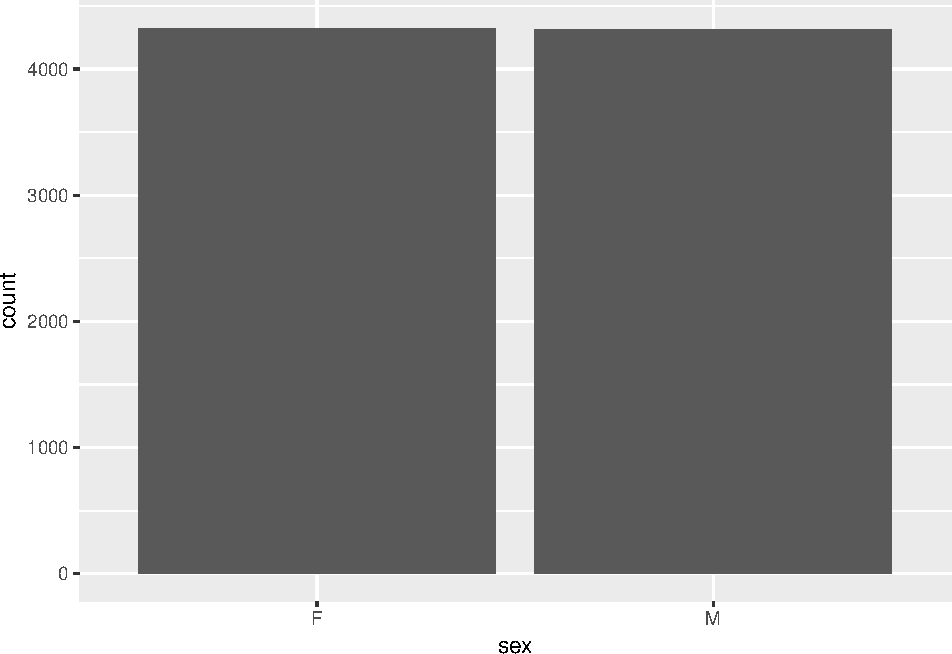
\includegraphics{_main_files/figure-latex/unnamed-chunk-4-1.pdf}

\subsection{Univariate - Continuous}\label{univariate---continuous}

A histogram looks very similar to a bar plot, but is used to represent
continuous data instead of categorical and therefore the bars will
actually be touching.

\begin{Shaded}
\begin{Highlighting}[]
\KeywordTok{ggplot}\NormalTok{(TenMileRace, }\KeywordTok{aes}\NormalTok{(}\DataTypeTok{x=}\NormalTok{net)) +}\StringTok{ }\KeywordTok{geom_histogram}\NormalTok{()}
\end{Highlighting}
\end{Shaded}

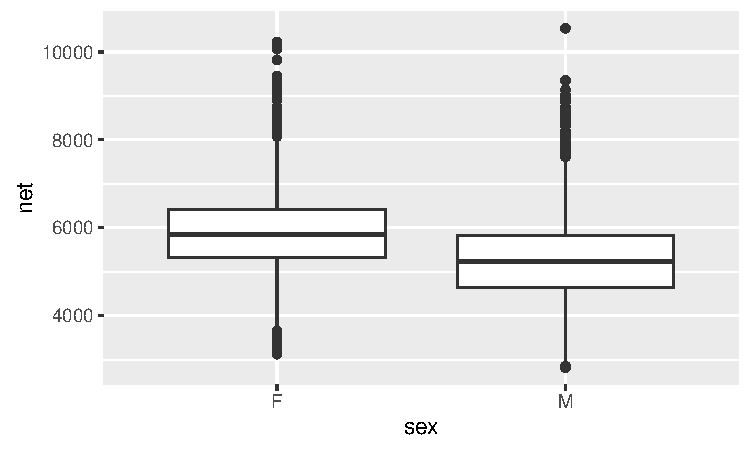
\includegraphics{_main_files/figure-latex/unnamed-chunk-5-1.pdf}

Often when a histogram is presented, the y-axis is labeled as
``frequency'' or ``count'' which is the number of observations that fall
within a particular bin. However, it is often desirable to scale the
y-axis so that if we were to sum up the area \((height * width)\) then
the total area would sum to 1. The rescaling that accomplishes this is
\[density=\frac{\#\;observations\;in\;bin}{total\;number\;observations}\cdot\frac{1}{bin\;width}\]

\subsection{Bivariate - Categorical vs
Continuous}\label{bivariate---categorical-vs-continuous}

We often wish to compare response levels from two or more groups of
interest. To do this, we often use side-by-side boxplots. Notice that
each observation is associated with a continuous response value and a
categorical value.

\begin{Shaded}
\begin{Highlighting}[]
\KeywordTok{ggplot}\NormalTok{(TenMileRace, }\KeywordTok{aes}\NormalTok{(}\DataTypeTok{x=}\NormalTok{sex, }\DataTypeTok{y=}\NormalTok{net)) +}\StringTok{ }\KeywordTok{geom_boxplot}\NormalTok{()}
\end{Highlighting}
\end{Shaded}

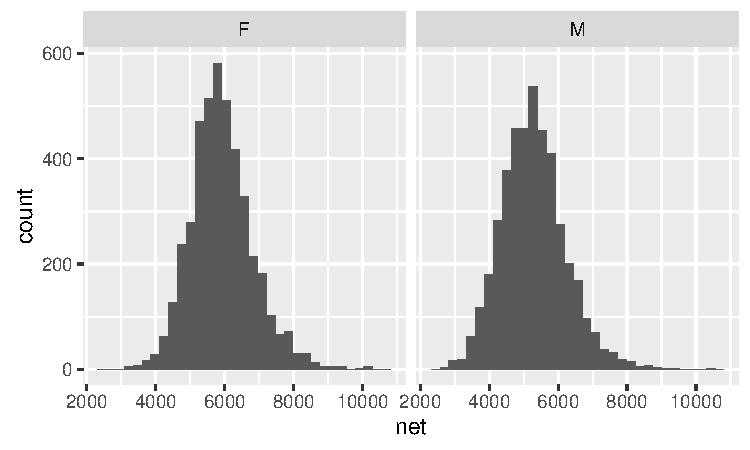
\includegraphics{_main_files/figure-latex/unnamed-chunk-6-1.pdf}

In this graph, the edges of the box are defined by the 25\% and 75\%
quantiles. That is to say, 25\% of the data is to the below of the box,
50\% of the data is in the box, and the final 25\% of the data is to the
above of the box. The dots are data points that traditionally considered
outliers.Define the Inter-Quartile Range (IQR) as the length of the box.
Then any observation more than 1.5*IQR from the box is considered an
outlier.

Sometimes I think that box-and-whisker plot obscures too much of the
details of the data and we should look at the side-by-side histograms
instead.

\begin{Shaded}
\begin{Highlighting}[]
\KeywordTok{ggplot}\NormalTok{(TenMileRace, }\KeywordTok{aes}\NormalTok{(}\DataTypeTok{x=}\NormalTok{net)) +}
\StringTok{  }\KeywordTok{geom_histogram}\NormalTok{() +}
\StringTok{  }\KeywordTok{facet_grid}\NormalTok{( . ~}\StringTok{ }\NormalTok{sex )  }\CommentTok{# side-by-side plots based on sex}
\end{Highlighting}
\end{Shaded}

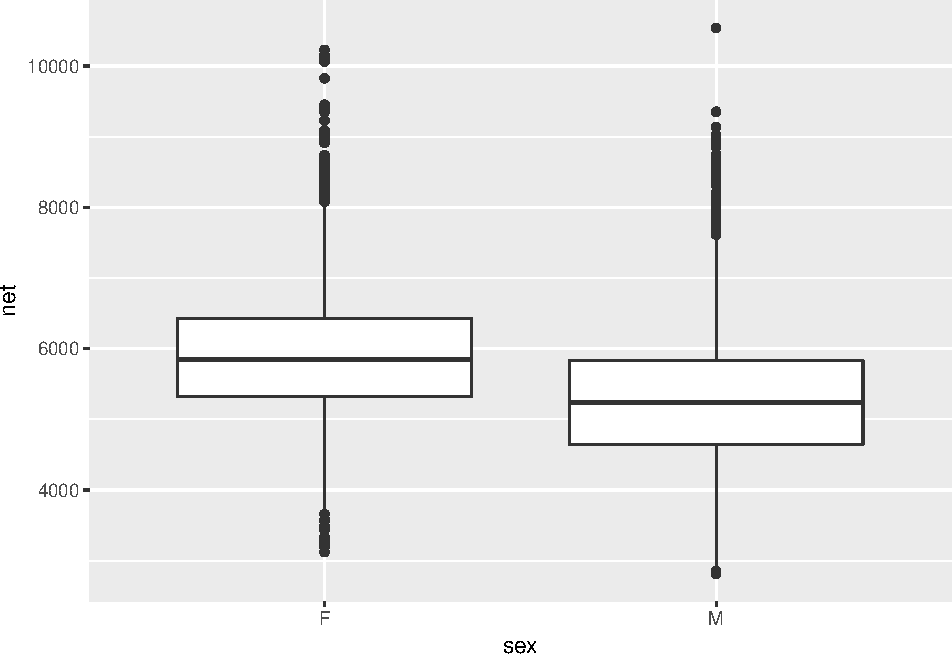
\includegraphics{_main_files/figure-latex/unnamed-chunk-7-1.pdf}

Orientation of graphs can certainly matter. In this case, it makes sense
to stack the two graphs to facilitate comparisons.

\begin{Shaded}
\begin{Highlighting}[]
\KeywordTok{ggplot}\NormalTok{(TenMileRace, }\KeywordTok{aes}\NormalTok{(}\DataTypeTok{x=}\NormalTok{net)) +}
\StringTok{  }\KeywordTok{geom_histogram}\NormalTok{() +}
\StringTok{  }\KeywordTok{facet_grid}\NormalTok{( sex ~}\StringTok{ }\NormalTok{. )  }\CommentTok{# side-by-side plots based on sex}
\end{Highlighting}
\end{Shaded}

\begin{verbatim}
## `stat_bin()` using `bins = 30`. Pick better value with `binwidth`.
\end{verbatim}

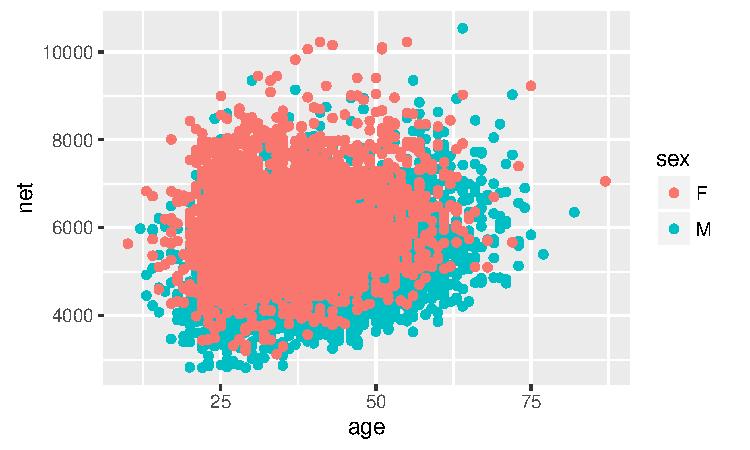
\includegraphics{_main_files/figure-latex/unnamed-chunk-8-1.pdf}

\subsection{Bivariate - Continuous vs
Continuous}\label{bivariate---continuous-vs-continuous}

Finally we might want to examine the relationship between two continuous
random variables.

\begin{Shaded}
\begin{Highlighting}[]
\KeywordTok{ggplot}\NormalTok{(TenMileRace, }\KeywordTok{aes}\NormalTok{(}\DataTypeTok{x=}\NormalTok{age, }\DataTypeTok{y=}\NormalTok{net, }\DataTypeTok{color=}\NormalTok{sex)) +}
\StringTok{  }\KeywordTok{geom_point}\NormalTok{()}
\end{Highlighting}
\end{Shaded}

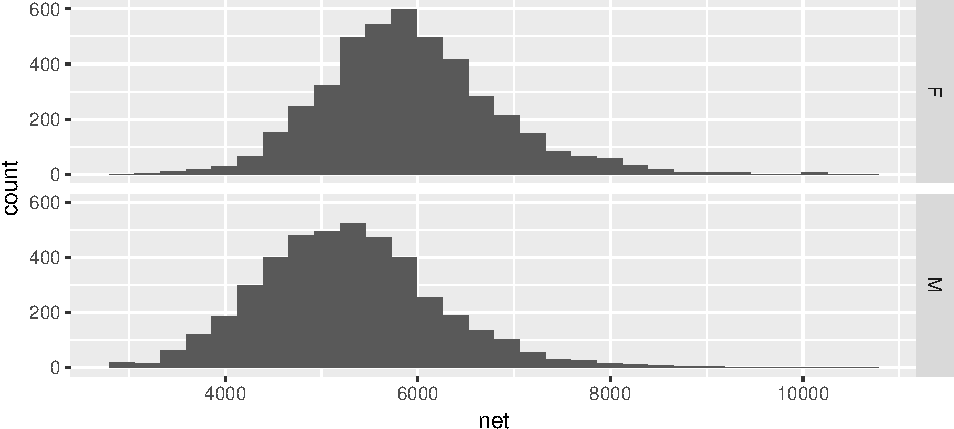
\includegraphics{_main_files/figure-latex/unnamed-chunk-9-1.pdf}

\section{Measures of Centrality}\label{measures-of-centrality}

The most basic question to ask of any dataset is `What is the typical
value?' There are several ways to answer that question and they should
be familiar to most students.

\subsection{Mean}\label{mean}

Often called the average, or arithmetic mean, we will denote this
special statistic with a bar. We define
\[\bar{x}=\frac{1}{n}\sum_{i=1}^{n}x_{i}=\frac{1}{n}\left(x_{1}+x_{2}+\dots+x_{n}\right)\]

If we want to find the mean of five numbers
\(\left\{ 3,6,4,8,2\right\}\) the calculation is
\[\bar{x}   =   \frac{1}{5}\left(3+6+4+8+2\right)
    =   \frac{1}{5}\left(23\right)
    =   23/5
    =   4.6\]

This can easily be calculated in R by using the function
\texttt{mean()}. We first extract the column we are interested in using
the notation: \texttt{DataSet\$ColumnName} where the \$ signifies
grabbing the column.

\begin{Shaded}
\begin{Highlighting}[]
\KeywordTok{mean}\NormalTok{( TenMileRace$net ) }\CommentTok{# Simplest way of doing this calculation}
\end{Highlighting}
\end{Shaded}

\begin{verbatim}
## [1] 5599.065
\end{verbatim}

\begin{Shaded}
\begin{Highlighting}[]
\NormalTok{TenMileRace %>%}\StringTok{ }\KeywordTok{summarise}\NormalTok{( }\KeywordTok{mean}\NormalTok{(net) )  }\CommentTok{# using the dplyr package}
\end{Highlighting}
\end{Shaded}

\begin{verbatim}
##   mean(net)
## 1  5599.065
\end{verbatim}

\subsection{Median}\label{median}

If the data were to be ordered, the median would be the middle most
observation (or, in the case that \(n\) is even, the mean of the two
middle most values).

In our simple case of five observations \(\left\{ 3,6,4,8,2\right\}\),
we first sort the data into \(\left\{ 2,3,4,6,8\right\}\) and then the
middle observation is clearly \(4\).

In R the median is easily calculated by the function \texttt{median()}.

\begin{Shaded}
\begin{Highlighting}[]
\CommentTok{# median( TenMileRace$net )}
\NormalTok{TenMileRace %>%}\StringTok{ }\KeywordTok{summarise}\NormalTok{( }\KeywordTok{median}\NormalTok{(net) ) }
\end{Highlighting}
\end{Shaded}

\begin{verbatim}
##   median(net)
## 1        5555
\end{verbatim}

\subsection{Mode}\label{mode}

This is the observation value with the most number of occurrences. This
measure of ``center'' is not often used

\subsection{Examples}\label{examples}

\begin{itemize}
\tightlist
\item
  If my father were to become bored with retirement and enroll in my STA
  570 course, how would that affect the mean and median age of my 570
  students?

  \begin{itemize}
  \tightlist
  \item
    The mean would move much more than the median. Suppose the class has
    5 people right now, ages 21, 22, 23, 23, 24 and therefore the median
    is 23. When my father joins, the ages will be 21, 22, 23, 23, 24, 72
    and the median will remain 23. However, the mean would move because
    we add in such a large outlier. Whenever we are dealing with skewed
    data, the mean is pulled toward the outlying observations.
  \end{itemize}
\item
  In 2010, the median NFL player salary was \$770,000 while the mean
  salary was \$1.9 million. Why the difference?

  \begin{itemize}
  \tightlist
  \item
    Because salary data is skewed superstar players that make huge
    salaries (in excess of 20 million) while the minimum salary for a
    rookie is \$375,000. Financial data often reflects a highly skewed
    distribution and the median is often a better measure of centrality
    in these cases.
  \end{itemize}
\end{itemize}

\section{Measures of Variation}\label{measures-of-variation}

The second question to ask of a dataset is `How much variability is
there?' Again there are several ways to measure that.

\subsection{Range}\label{range}

Range is the distance from the largest to the smallest value in the
dataset.

\begin{Shaded}
\begin{Highlighting}[]
\CommentTok{#vmax( TenMileRace$net ) - min( TenMileRace$net )}
\NormalTok{TenMileRace %>%}\StringTok{ }\KeywordTok{summarise}\NormalTok{( }\DataTypeTok{range =} \KeywordTok{max}\NormalTok{(net) -}\StringTok{ }\KeywordTok{min}\NormalTok{(net) )}
\end{Highlighting}
\end{Shaded}

\begin{verbatim}
##   range
## 1  7722
\end{verbatim}

\subsection{Inter-Quartile Range}\label{inter-quartile-range}

The p-th percentile is the observation (or observations) that has at
most \(p\) percent of the observations below it and \((1-p)\) above it,
where \(p\) is between 0 and 100. The median is the \(50\)th percentile.
Often we are interested in splitting the data into four equal sections
using the \(25\)th, \(50\)th, and \(75\)th percentiles (which, because
it splits the data into four sections, we often call these the \(1\)st,
\(2\)nd, and \(3\)rd quartiles).

In general I could be interested in dividing my data up into an
arbitrary number of sections, and refer to those as quantiles of my
data.

\begin{Shaded}
\begin{Highlighting}[]
\KeywordTok{quantile}\NormalTok{( TenMileRace$net ) }\CommentTok{# this works}
\end{Highlighting}
\end{Shaded}

\begin{verbatim}
##    0%   25%   50%   75%  100% 
##  2814  4950  5555  6169 10536
\end{verbatim}

\begin{Shaded}
\begin{Highlighting}[]
\CommentTok{# I can't do the following because the quantile() function spits out 5 values, not 1}
\CommentTok{# TenMileRace %>% summarise( quantile(net) )  }
\end{Highlighting}
\end{Shaded}

The inter-quartile range (IQR) is defined as the distance from the
\(3\)rd quartile to the \(1\)st.

\begin{Shaded}
\begin{Highlighting}[]
\CommentTok{# IQR( TenMileRace$net )}
\NormalTok{TenMileRace %>%}\StringTok{ }\KeywordTok{summarise}\NormalTok{( }\KeywordTok{IQR}\NormalTok{(net) ) }
\end{Highlighting}
\end{Shaded}

\begin{verbatim}
##   IQR(net)
## 1     1219
\end{verbatim}

Notice that we've defined IQR before when we looked at box-and-whisker
plots and this is exactly the length of the box.

\subsection{Variance}\label{variance}

One way to measure the spread of a distribution is to ask ``what is the
typical distance of an observation to the mean?'' We could define the
\(i\)th deviate as \[e_{i}=x_{i}-\bar{x}\] and then ask what is the
average deviate? The problem with this approach is that the sum (and
thus the average) of all deviates is always 0.
\[\sum_{i=1}^{n}(x_{i}-\bar{x}) =   \sum_{i=1}^{n}x_{i}-\sum_{i=1}^{n}\bar{x}
    =   n\frac{1}{n}\sum_{i=1}^{n}x_{i}-n\bar{x}
    =   n\bar{x}-n\bar{x}
    =   0\]

The big problem is that about half the deviates are negative and the
others are positive. What we really care is the distance from the mean,
not the sign. So we could either take the absolute value, or square it.

There are some really good theoretical reasons to chose the square
option. Squared terms are easier to deal with compared to absolute
values, but more importantly, the spread of the normal distribution is
parameterized via squared distances from the mean. Because the normal
distribution is so important, we've chosen to define the sample variance
so it matches up with the natural spread parameter of the normal
distribution. So we square the deviates and then find the average
deviate size (approximately) and call that the sample variance.
\[s^{2}=\frac{1}{n-1}\sum_{i=1}^{n}\left(x_{i}-\bar{x}\right)^{2}\] Why
do we divide by \(n-1\) instead of \(n\)?

\begin{enumerate}
\def\labelenumi{\arabic{enumi}.}
\tightlist
\item
  If I divide by \(n\), then on average, we would tend to underestimate
  the population variance \(\sigma^{2}\).
\item
  The reason is because we are using the same set of data to estimate
  \(\sigma^{2}\) as we did to estimate the population mean (\(\mu\)). If
  I could use\\
  \[\frac{1}{n}\sum_{i=1}^{n}\left(x_{i}-\mu\right)^{2}\] as my
  estimator, we would be fine. But because I have to replace \(\mu\)
  with \(\bar{x}\) we have to pay a price.
\item
  Because the estimation of \(\sigma^{2}\) requires the estimation of
  one other quantity, and using using that quantity, you only need
  \(n-1\) data points and can then figure out the last one, we have used
  one degree of freedom on estimating the mean and we need to adjust the
  formula accordingly.
\end{enumerate}

In later chapters we'll give this quantity a different name, so we'll
introduce the necessary vocabulary here. Let \(e_{i}=x_{i}-\bar{x}\) be
the error left after fitting the sample mean. This is the deviation from
the observed value to the ``expected value'' \(\bar{x}\). We can then
define the Sum of Squared Error as \[SSE=\sum_{i=1}^{n}e_{i}^{2}\]

and the Mean Squared Error as
\[MSE=\frac{SSE}{df}=\frac{SSE}{n-1}=s^{2}\] where \(df=n-1\) is the
appropriate degrees of freedom.

Calculating the variance of our small sample of five observations
\(\left\{ 3,6,4,8,2\right\}\), recall that the sample mean was
\(\bar{x}=4.6\)

\begin{longtable}[]{@{}lll@{}}
\toprule
\(x_i\) & \((x_i-\bar{x})\) & \((x_i-\bar{x})^2\)\tabularnewline
\midrule
\endhead
3 & -1.6 & 2.56\tabularnewline
6 & 1.4 & 1.96\tabularnewline
4 & -0.6 & 0.36\tabularnewline
8 & 3.4 & 11.56\tabularnewline
2 & -2.6 & 6.76\tabularnewline
-------- & ------------------- & --------------------\tabularnewline
& SSE = 23.2\tabularnewline
\bottomrule
\end{longtable}

and so the sample variance is
\[s^2 = \frac{23.2}{(n-1)} = \frac{23.2}{4}=5.8\]

Clearly this calculation would get very tedious to do by hand and
computers will be much more accurate in these calculations. In R, the
sample variance is easily calculated by the function var().

\begin{Shaded}
\begin{Highlighting}[]
\NormalTok{ToyData <-}\StringTok{ }\KeywordTok{data.frame}\NormalTok{( }\DataTypeTok{x=}\KeywordTok{c}\NormalTok{(}\DecValTok{3}\NormalTok{,}\DecValTok{6}\NormalTok{,}\DecValTok{4}\NormalTok{,}\DecValTok{8}\NormalTok{,}\DecValTok{2}\NormalTok{) )}
\CommentTok{# var( ToyData$x )}
\NormalTok{ToyData %>%}\StringTok{ }\KeywordTok{summarise}\NormalTok{( }\DataTypeTok{s2 =} \KeywordTok{var}\NormalTok{(x) )}
\end{Highlighting}
\end{Shaded}

\begin{verbatim}
##    s2
## 1 5.8
\end{verbatim}

For the larger TenMileRace data set, the variance is just as easily
calculated.

\begin{Shaded}
\begin{Highlighting}[]
\CommentTok{# var( TenMileRace$net )}
\NormalTok{TenMileRace %>%}\StringTok{ }\KeywordTok{summarise}\NormalTok{( }\DataTypeTok{s2 =} \KeywordTok{var}\NormalTok{(net) )}
\end{Highlighting}
\end{Shaded}

\begin{verbatim}
##         s2
## 1 940233.5
\end{verbatim}

\subsection{Standard Deviation}\label{standard-deviation}

The biggest problem with the sample variance statistic is that the units
are in the original units-squared. That means if you are looking at data
about car fuel efficiency, then the values would be in mpg\(^{2}\) which
are units that I can't really understand. The solution is to take the
positive square root, which we will call the sample standard deviation.
\[s=\sqrt{s^{2}}\] But why do we take the jog through through variance?
Mathematically the variance is more useful and most distributions (such
as the normal) are defined by the variance term. Practically though,
standard deviation is easier to think about.

The sample standard deviation is important enough for R to have function
that will calculate it for you.

\begin{Shaded}
\begin{Highlighting}[]
\CommentTok{# sd( TenMileRace$net )}
\NormalTok{TenMileRace %>%}\StringTok{ }\KeywordTok{summarise}\NormalTok{( }\DataTypeTok{s =} \KeywordTok{sd}\NormalTok{(net) )}
\end{Highlighting}
\end{Shaded}

\begin{verbatim}
##          s
## 1 969.6564
\end{verbatim}

\subsection{Coefficient of Variation}\label{coefficient-of-variation}

Suppose we had a group of animals and the sample standard deviation of
the animals lengths was 15 cm. If the animals were elephants, you would
be amazed at their uniformity in size, but if they were insects, you
would be astounded at the variability. To account for that, the
coefficient of variation takes the sample standard deviation and divides
by the absolute value of the sample mean (to keep everything positive)

\[CV=\frac{s}{\vert\bar{x}\vert}\]

\begin{Shaded}
\begin{Highlighting}[]
\NormalTok{TenMileRace %>%}\StringTok{ }\KeywordTok{summarise}\NormalTok{( }\DataTypeTok{s =} \KeywordTok{sd}\NormalTok{(net),}
                           \DataTypeTok{xbar =} \KeywordTok{mean}\NormalTok{(net),}
                           \DataTypeTok{cv =} \NormalTok{s /}\StringTok{ }\KeywordTok{abs}\NormalTok{(xbar) )}
\end{Highlighting}
\end{Shaded}

\begin{verbatim}
##          s     xbar        cv
## 1 969.6564 5599.065 0.1731818
\end{verbatim}

\begin{Shaded}
\begin{Highlighting}[]
\CommentTok{# For fun, lets calculate these same statistics but separated by sex...}
\NormalTok{TenMileRace %>%}\StringTok{ }
\StringTok{  }\KeywordTok{group_by}\NormalTok{(sex) %>%}
\StringTok{  }\KeywordTok{summarise}\NormalTok{( }\DataTypeTok{xbar =} \KeywordTok{mean}\NormalTok{(net),}
             \DataTypeTok{s    =} \KeywordTok{sd}\NormalTok{(net),}
             \DataTypeTok{cv   =} \NormalTok{s /}\StringTok{ }\KeywordTok{abs}\NormalTok{(xbar) )}
\end{Highlighting}
\end{Shaded}

\begin{verbatim}
## # A tibble: 2 × 4
##      sex     xbar        s        cv
##   <fctr>    <dbl>    <dbl>     <dbl>
## 1      F 5916.398 902.1090 0.1524761
## 2      M 5280.702 929.9817 0.1761095
\end{verbatim}

\subsection{Empirical Rule of Thumb}\label{empirical-rule-of-thumb}

For any mound-shaped sample of data the following is a reasonable rule
of thumb:

\begin{longtable}[]{@{}ll@{}}
\toprule
Interval & Approximate percent of Measurements\tabularnewline
\midrule
\endhead
\(\bar{x}\pm s\) & 68\%\tabularnewline
\(\bar{x}\pm 2s\) & 95\%\tabularnewline
\(\bar{x}\pm 3s\) & 99.7\%\tabularnewline
\bottomrule
\end{longtable}

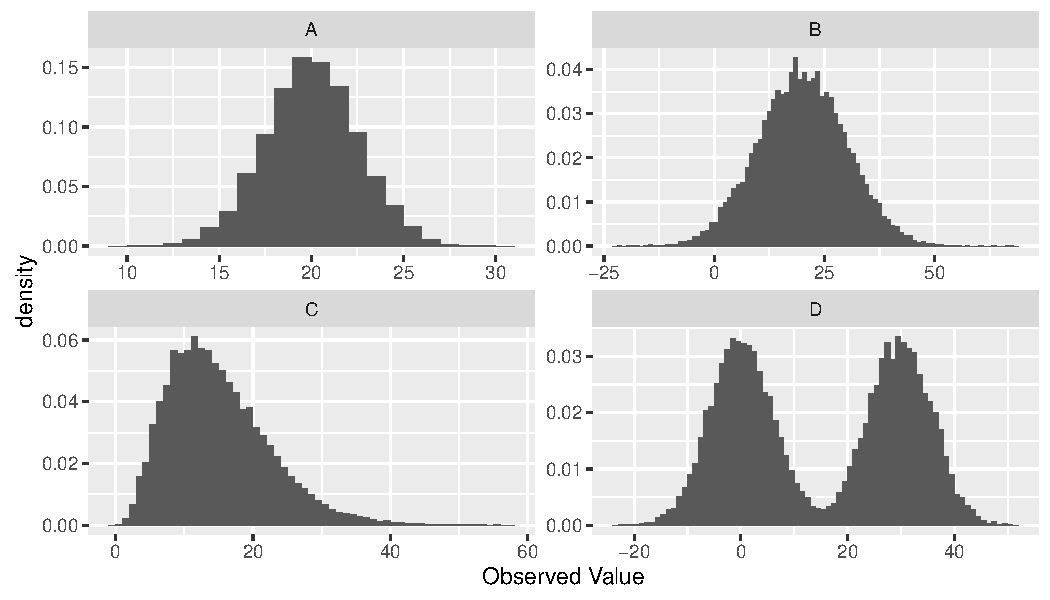
\includegraphics{_main_files/figure-latex/unnamed-chunk-20-1.pdf}

\section{Exercises}\label{exercises}

\begin{enumerate}
\def\labelenumi{\arabic{enumi}.}
\item
  O\&L 3.21. The ratio of DDE (related to DDT) to PCB concentrations in
  bird eggs has been shown to have had a number of biological
  implications. The ratio is used as an indication of the movement of
  contamination through the food chain. The paper ``The ratio of DDE to
  PCB concentrations in Great Lakes herring gull eggs and its us in
  interpreting contaminants data'' reports the following ratios for eggs
  collected at 13 study sites from the five Great Lakes. The eggs were
  collected from both terrestrial and aquatic feeding birds.

  \begin{longtable}[]{@{}ll@{}}
  \toprule
  \begin{minipage}[t]{0.20\columnwidth}\raggedright\strut
  Source Type\strut
  \end{minipage} &
  \begin{minipage}[t]{0.74\columnwidth}\raggedright\strut
  DDE to PCB Ratio\strut
  \end{minipage}\tabularnewline
  \begin{minipage}[t]{0.20\columnwidth}\raggedright\strut
  \textbf{Terrestrial} \textbf{Aquatic}\strut
  \end{minipage} &
  \begin{minipage}[t]{0.74\columnwidth}\raggedright\strut
  76.50, 6.03, 3.51, 9.96, 4.24, 7.74, 9.54, 41.70, 1.84, 2.5, 1.54
  0.27, 0.61, 0.54, 0.14, 0.63, 0.23, 0.56, 0.48, 0.16, 0.18\strut
  \end{minipage}\tabularnewline
  \bottomrule
  \end{longtable}

  \begin{enumerate}
  \def\labelenumii{\alph{enumii})}
  \tightlist
  \item
    By hand, compute the mean and median separately for each type of
    feeder.
  \item
    Using your results from part (a), comment on the relative
    sensitivity of the mean and median to extreme values in a data set.
  \item
    Which measure, mean or median, would you recommend as the most
    appropriate measure of the DDE to PCB level for both types of
    feeders? Explain your answer.
  \end{enumerate}
\item
  O\&L 3.31. Consumer Reports in its June 1998 issue reports on the
  typical daily room rate at six luxury and nine budget hotels. The room
  rates are given in the following table.

  \begin{longtable}[]{@{}ll@{}}
  \toprule
  Hotel Type & Nightly Rate\tabularnewline
  \midrule
  \endhead
  Luxury & \$175, \$180, \$120, \$150, \$120, \$125\tabularnewline
  Budget & \$50, \$50, \$49, \$45, \$36, \$45, \$50, \$50,
  \$40\tabularnewline
  \bottomrule
  \end{longtable}

  \begin{enumerate}
  \def\labelenumii{\alph{enumii})}
  \tightlist
  \item
    By hand, compute the means and standard deviations of the room rates
    for each class of hotel.
  \item
    Give a practical reason why luxury hotels might have higher
    variability than the budget hotels. (Don't just say the standard
    deviation is higher because there is more spread in the data, but
    rather think about the Hotel Industry and why you might see greater
    price variability for upscale goods compared to budget items.)
  \end{enumerate}
\item
  Use R to confirm your calculations in problem 1 (the pollution data).
  Show the code you used and the subsequent output. It will often be
  convenient for me to give you code that generates a data frame instead
  of uploading an Excel file and having you read it in. The data can be
  generated using the following commands:

\begin{Shaded}
\begin{Highlighting}[]
\NormalTok{PolutionRatios <-}\StringTok{ }\KeywordTok{data.frame}\NormalTok{(}
  \DataTypeTok{Ratio =} \KeywordTok{c}\NormalTok{(}\FloatTok{76.50}\NormalTok{, }\FloatTok{6.03}\NormalTok{, }\FloatTok{3.51}\NormalTok{, }\FloatTok{9.96}\NormalTok{, }\FloatTok{4.24}\NormalTok{, }\FloatTok{7.74}\NormalTok{, }\FloatTok{9.54}\NormalTok{, }\FloatTok{41.70}\NormalTok{, }\FloatTok{1.84}\NormalTok{, }\FloatTok{2.5}\NormalTok{, }\FloatTok{1.54}\NormalTok{,}
             \FloatTok{0.27}\NormalTok{, }\FloatTok{0.61}\NormalTok{, }\FloatTok{0.54}\NormalTok{, }\FloatTok{0.14}\NormalTok{, }\FloatTok{0.63}\NormalTok{, }\FloatTok{0.23}\NormalTok{, }\FloatTok{0.56}\NormalTok{,  }\FloatTok{0.48}\NormalTok{, }\FloatTok{0.16}\NormalTok{, }\FloatTok{0.18}       \NormalTok{),}
  \DataTypeTok{Type  =} \KeywordTok{c}\NormalTok{( }\KeywordTok{rep}\NormalTok{(}\StringTok{'Terrestrial'}\NormalTok{,}\DecValTok{11}\NormalTok{), }\KeywordTok{rep}\NormalTok{(}\StringTok{'Aquatic'}\NormalTok{,}\DecValTok{10}\NormalTok{) ) )}

\CommentTok{# Print out some of the data to confirm what the column names are}
\KeywordTok{head}\NormalTok{( PolutionRatios )}
\end{Highlighting}
\end{Shaded}

\begin{verbatim}
##   Ratio        Type
## 1 76.50 Terrestrial
## 2  6.03 Terrestrial
## 3  3.51 Terrestrial
## 4  9.96 Terrestrial
## 5  4.24 Terrestrial
## 6  7.74 Terrestrial
\end{verbatim}

  \emph{Hint: for computing the means and medians for each type of
  feeder separately, the \texttt{group\_by()} command we demonstated
  earlier in the chapter is convenient.}
\item
  Use R to confirm your calculations in problem 2 (the hotel data). Show
  the code you used and the subsequent output. The data can be loaded
  into a data frame using the following commands Show the code you used
  and the subsequent output:

\begin{Shaded}
\begin{Highlighting}[]
\NormalTok{Hotels <-}\StringTok{ }\KeywordTok{data.frame}\NormalTok{(}
  \DataTypeTok{Price =} \KeywordTok{c}\NormalTok{(}\DecValTok{175}\NormalTok{, }\DecValTok{180}\NormalTok{, }\DecValTok{120}\NormalTok{, }\DecValTok{150}\NormalTok{, }\DecValTok{120}\NormalTok{, }\DecValTok{125}\NormalTok{, }\DecValTok{50}\NormalTok{, }\DecValTok{50}\NormalTok{, }\DecValTok{49}\NormalTok{, }\DecValTok{45}\NormalTok{, }\DecValTok{36}\NormalTok{, }\DecValTok{45}\NormalTok{, }\DecValTok{50}\NormalTok{, }\DecValTok{50}\NormalTok{, }\DecValTok{40}\NormalTok{),}
  \DataTypeTok{Type  =} \KeywordTok{c}\NormalTok{( }\KeywordTok{rep}\NormalTok{(}\StringTok{'Luxury'}\NormalTok{,}\DecValTok{6}\NormalTok{),  }\KeywordTok{rep}\NormalTok{(}\StringTok{'Budget'}\NormalTok{, }\DecValTok{9}\NormalTok{) ) )}

\CommentTok{# Print out some of the data to confirm what the column names are}
\KeywordTok{head}\NormalTok{( Hotels )}
\end{Highlighting}
\end{Shaded}

\begin{verbatim}
##   Price   Type
## 1   175 Luxury
## 2   180 Luxury
## 3   120 Luxury
## 4   150 Luxury
## 5   120 Luxury
## 6   125 Luxury
\end{verbatim}
\item
  For the hotel data, create side-by-side box-and-whisker plots to
  compare the prices.
\item
  Match the following histograms to the appropriate boxplot.
  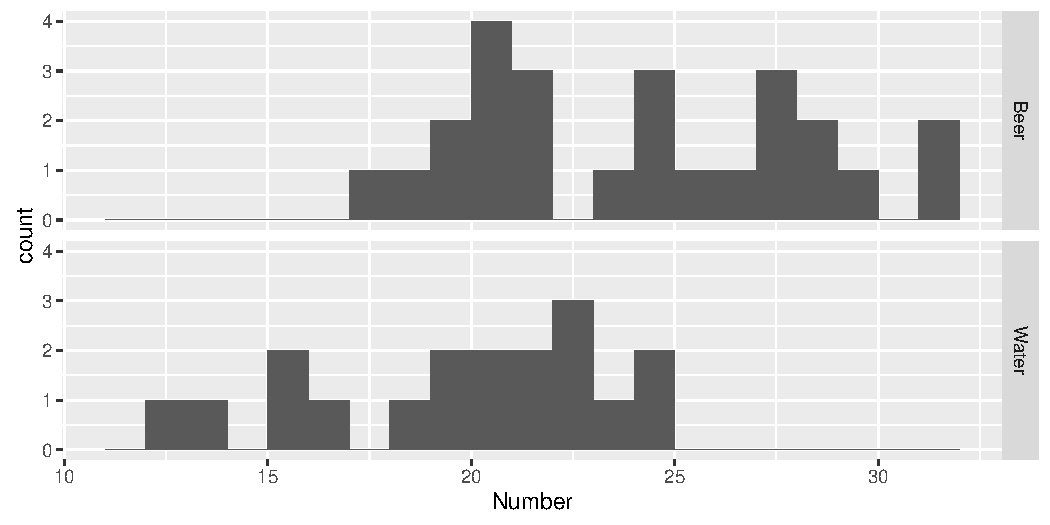
\includegraphics{_main_files/figure-latex/unnamed-chunk-23-1.pdf}
  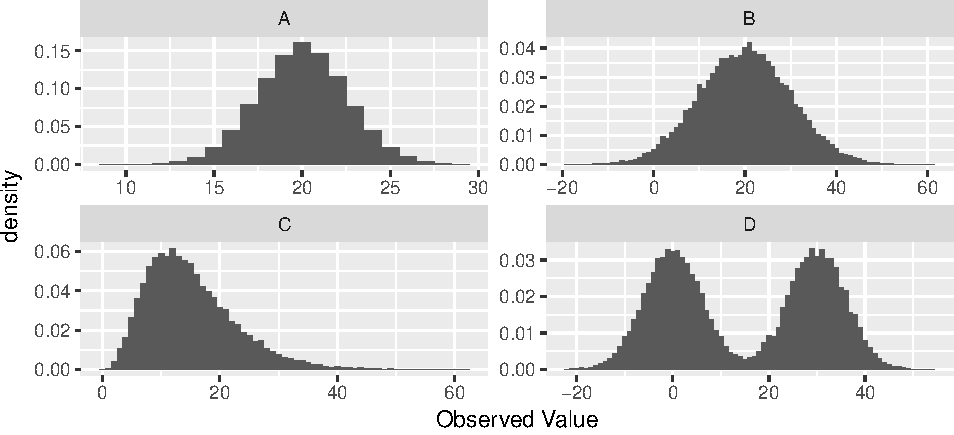
\includegraphics{_main_files/figure-latex/unnamed-chunk-24-1.pdf}

  \begin{enumerate}
  \def\labelenumii{\alph{enumii})}
  \tightlist
  \item
    Histogram A goes with boxplot \_\_\_\_\_\_\_\_\_\_
  \item
    Histogram B goes with boxplot \_\_\_\_\_\_\_\_\_\_
  \item
    Histogram C goes with boxplot \_\_\_\_\_\_\_\_\_\_
  \item
    Histogram D goes with boxplot \_\_\_\_\_\_\_\_\_\_
  \end{enumerate}
\item
  Twenty-five employees of a corporation have a mean salary of \$62,000
  and the sample standard deviation of those salaries is \$15,000. If
  each employee receives a bonus of \$1,000, does the standard deviation
  of the salaries change? Explain your reasoning.
\end{enumerate}

\chapter{Probability}\label{probability}

\begin{Shaded}
\begin{Highlighting}[]
\CommentTok{# Every chapter, we will load all the librarys we will use at the beginning}
\CommentTok{# of the chapter. }
\KeywordTok{library}\NormalTok{(ggplot2)    }\CommentTok{# graphing functions}
\KeywordTok{library}\NormalTok{(dplyr)      }\CommentTok{# data summary tools}
\end{Highlighting}
\end{Shaded}

We need to work out the mathematics of what we mean by probability. To
begin with we first define an outcome. An outcome is one observation
from a random process or event. For example we might be interested in a
single roll of a six-side die. Alternatively we might be interested in
selecting one NAU student at random from the entire population of NAU
students.

\section{Introduction to Set Theory}\label{introduction-to-set-theory}

Before we jump into probability, it is useful to review a little bit of
set theory.

Events are properties of a particular outcome. For a coin flip, the
event ``Heads'' would be the event that a heads was flipped. For the
single roll of a six-sided die, a possible event might be that the
result is even. For the NAU student, we might be interested in the event
that the student is a biology student. A second event of interest might
be if the student is an undergraduate.

1.1.1 Venn Diagrams

Let \(S\) be the set of all outcomes of my random trial. Suppose I am
interested in two events \(A\) and \(B\). The traditional way of
representing these events is using a Venn diagram.

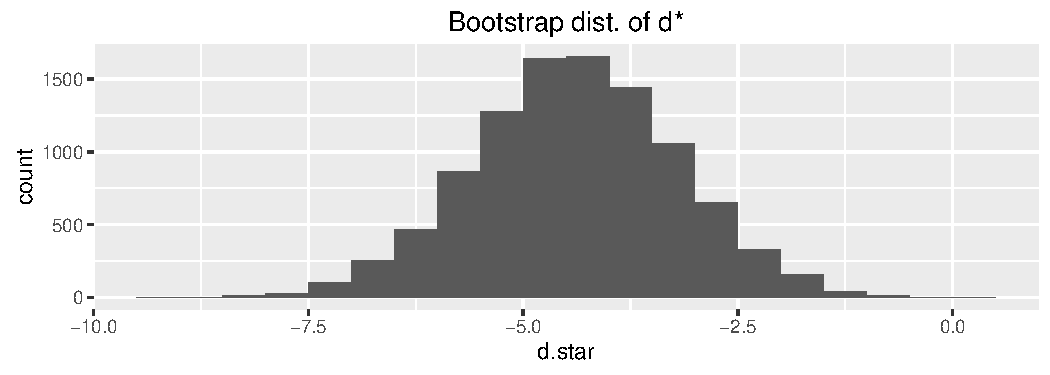
\includegraphics{_main_files/figure-latex/unnamed-chunk-27-1.pdf}

For example, suppose that my random experiment is rolling a fair 6-sided
die once. The possible outcomes are \(S=\{1,2,3,4,5,6\}\). Suppose I
then define events \(A=\) roll is odd and \(B=\) roll is 5 or greater.
In this case our picture is:

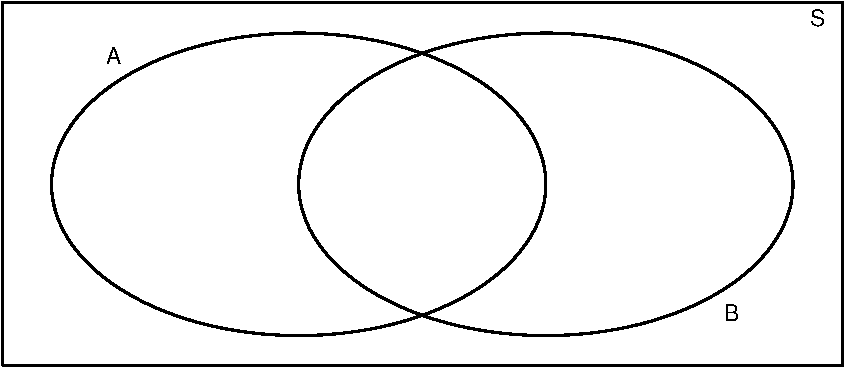
\includegraphics{_main_files/figure-latex/unnamed-chunk-28-1.pdf}

All of our possible events are present, and distributed amongst our
possible events.

1.1.2 Composition of events

I am often interested in discussing the composition of two events and we
give the common set operations below.

\begin{itemize}
\item
  Union: Denote the event that either \(A\) or \(B\) occurs as
  \(A\cup B\).
  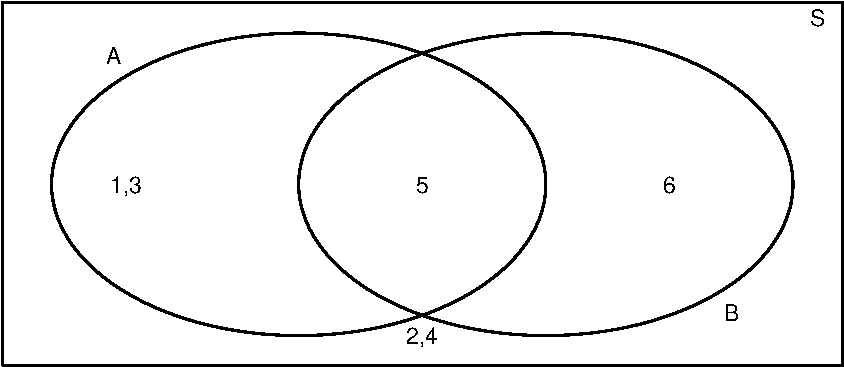
\includegraphics{_main_files/figure-latex/unnamed-chunk-29-1.pdf}
\item
  Denote the event that \textbf{both} \(A\) and \(B\) occur as
  \(A\cap B\)
  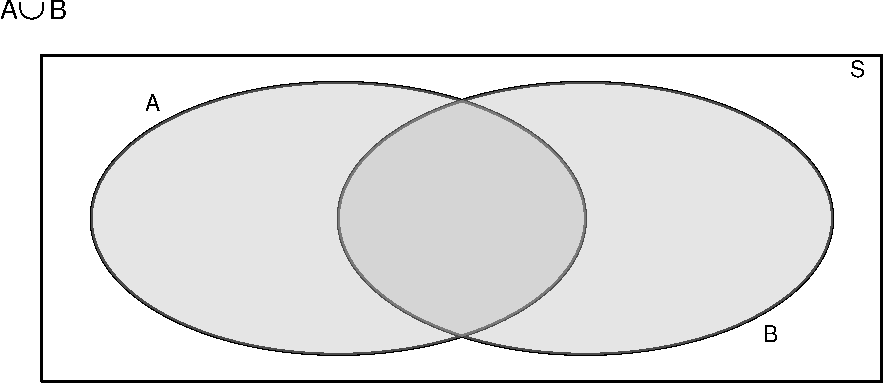
\includegraphics{_main_files/figure-latex/unnamed-chunk-30-1.pdf}
\item
  Denote the event that \(A\) does not occur as \(\bar{A}\) or \(A^{C}\)
  (different people use different notations)
  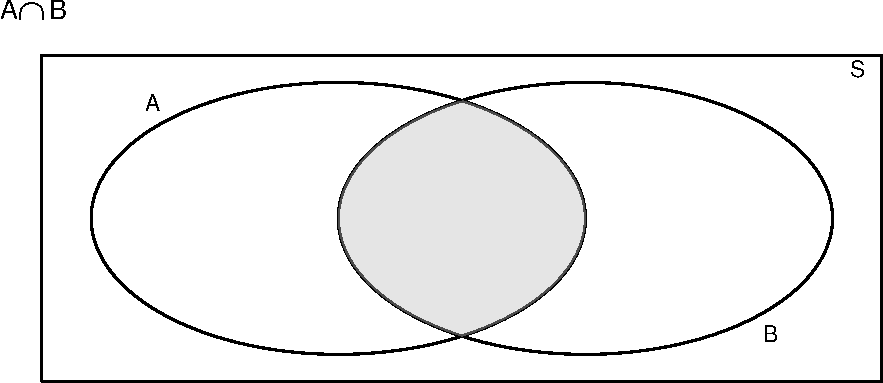
\includegraphics{_main_files/figure-latex/unnamed-chunk-31-1.pdf}
\end{itemize}

\textbf{Definition 1}. Two events \(A\) and \(B\) are said to be
mutually exclusive (or disjoint) if the occurrence of one event
precludes the occurrence of the other. For example, on a single roll of
a die, a two and a five cannot both come up. For a second example,
define \(A\) to be the event that the die is even, and \(B\) to be the
event that the die comes up as a \(5\).

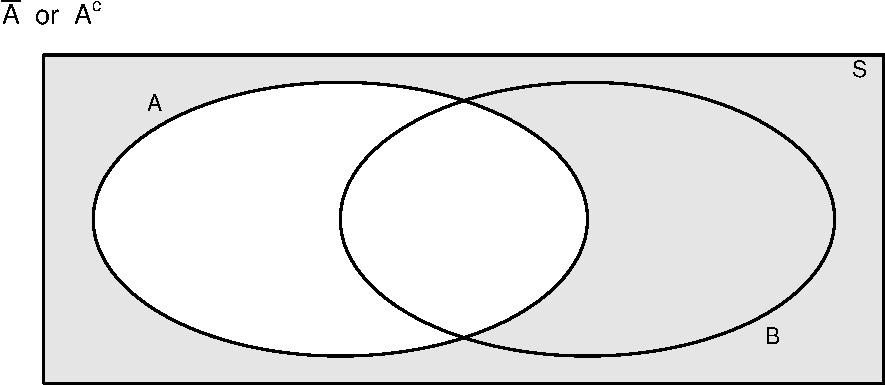
\includegraphics{_main_files/figure-latex/unnamed-chunk-32-1.pdf}

\section{Probability Rules}\label{probability-rules}

\subsection{Simple Rules}\label{simple-rules}

We now take our Venn diagrams and use them to understand the rules of
probability. The underlying idea that we will use is the the probability
of an event is the area in the Venn diagram.

\textbf{Definition 2}. Probability is the proportion of times an event
occurs in many repeated trials of a random phenomenon. In other words,
probability is the long-term relative frequency.

\textbf{Fact}. \emph{For any event \(A\) the probability of the event
\(P(A)\) satisfies \(0\le P(A) \le 1\) because proportions always lie in
\([0,1]\).}

Because \(S\) is the set of all events that might occur, the area of our
bounding rectangle will be \(1\) and the probability of event \(A\)
occurring will be represented by the area in the circle \(A\).

\textbf{Fact}. \emph{If two events are mutually exclusive, then
\(P(A\cup B)=P(A)+P(B)\)}

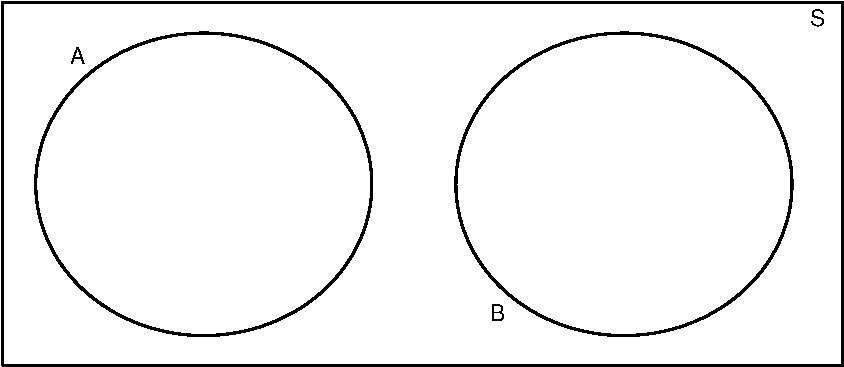
\includegraphics{_main_files/figure-latex/unnamed-chunk-33-1.pdf}

\textbf{Example}. Let \(R\) be the sum of two different colored dice.
Suppose we are interested in \(P(R \le 4)\). Notice that the pair of
dice can fall 36 different ways (6 ways for the first die and six for
the second results in 6x6 possible outcomes, and each way has equal
probability \(1/36\). Because the dice cannot simultaneously sum to
\(2\) and to \(3\), we could write P(R \le 4 ) = P(R=2)+P(R=3)+P(R=4) =
P(\left\{ 1,1\right\} )+P(\left\{ 1,2\right\}
\mathrm{\textrm{ or }}\left\{ 2,1\right\}
)+P(\{1,3\}\textrm{ or }\{2,2\}\textrm{ or }\{3,1\}) =
\frac{1}{36}+\frac{2}{36}+\frac{3}{36} = \frac{6}{36} = \frac{1}{6}

\textbf{Fact}. \(P(A)+P(\bar{A})=1\)
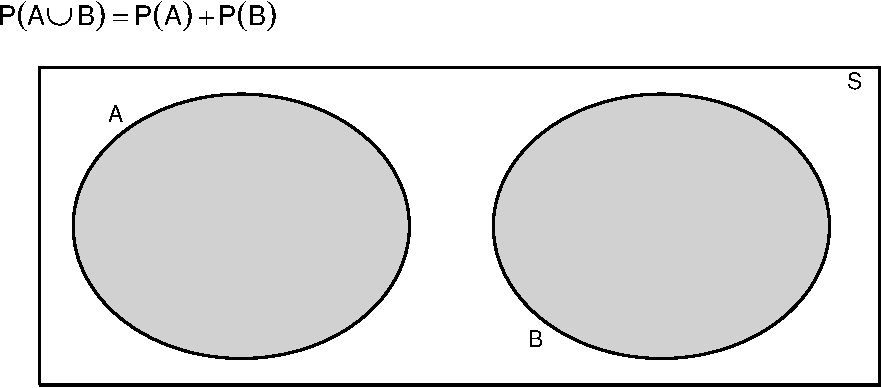
\includegraphics{_main_files/figure-latex/unnamed-chunk-34-1.pdf}

The above statement is true because the probability of whole space \(S\)
is one (remember \(S\) is all possible outcomes), then either we get an
outcome in which \(A\) occurs or we get an outcome in which \(A\) does
not occur.

\textbf{Fact}. \(P(A\cup B)=P(A)+P(B)-P(A\cap B)\)

The reason behind this fact is that if there is if \(A\) and \(B\) are
not disjoint, then some area is added twice when I calculate
\(P\left(A\right)+P\left(B\right)\). To account for this, I simply
subtract off the area that was double counted.

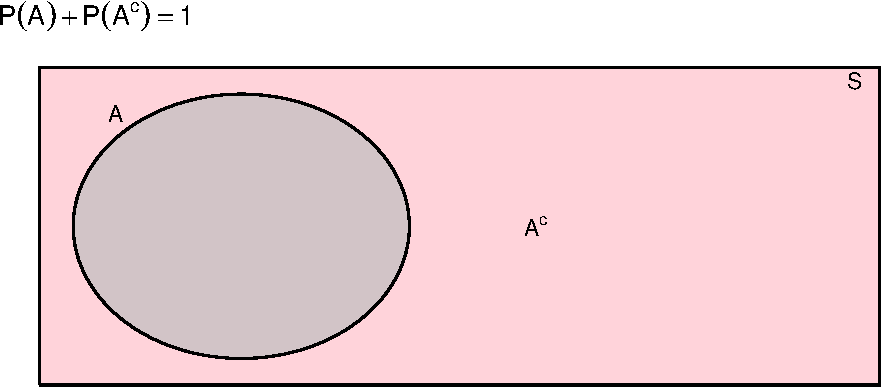
\includegraphics{_main_files/figure-latex/unnamed-chunk-35-1.pdf}

\textbf{Fact 3}. \(P(A)=P(A\cap B)+P(A\cap\bar{B})\)

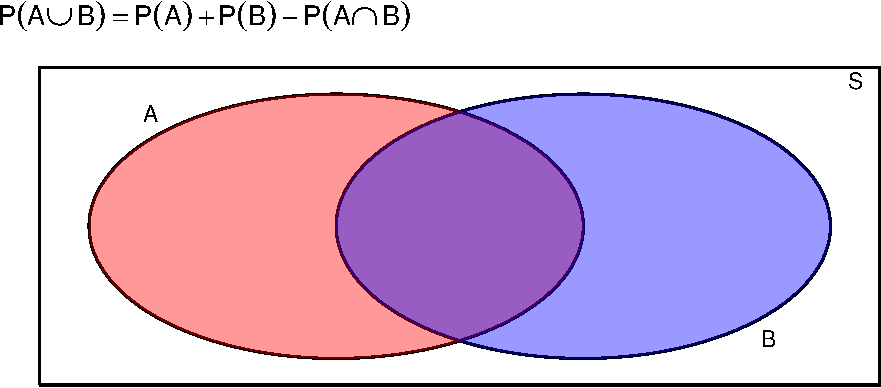
\includegraphics{_main_files/figure-latex/unnamed-chunk-36-1.pdf}

This identity is just breaking the event \(A\) into two disjoint pieces.

\subsection{Conditional Probability}\label{conditional-probability}

We are given the following data about insurance claims. Notice that the
data is given as \(P(\;Category\;\cap\;PolicyType\;)\) which is apparent
because the sum of all the elements in the table is \(100\%\)

\begin{longtable}[]{@{}llll@{}}
\toprule
\(\,\) & Fire & Auto & Other\tabularnewline
\midrule
\endhead
\textbf{Fraudulant} & 6\% & 1\% & 3\%\tabularnewline
\textbf{non-Fraudulant} & 14\% & 29\% & 47\%\tabularnewline
\bottomrule
\end{longtable}

Summing across the rows and columns, we can find the probabilities of
for each category and policy type.

\begin{longtable}[]{@{}lllll@{}}
\toprule
\(\,\) & Fire & Auto & Other & \(\,\)\tabularnewline
\midrule
\endhead
\textbf{Fraudulant} & 6\% & 1\% & 3\% & \textbf{10\%}\tabularnewline
\textbf{non-Fraudulant} & 14\% & 29\% & 47\% &
\textbf{90\%}\tabularnewline
\(\,\) & \textbf{20\%} & \textbf{30\%} & \textbf{50\%} &
\textbf{100\%}\tabularnewline
\bottomrule
\end{longtable}

It is clear that fire claims are more likely fraudulent than auto or
other claims. In fact, the proportion of fraudulent claims, given that
the claim is against a fire policy is \[\begin{aligned}
P(\textrm{ Fraud }|\textrm{ FirePolicy })   &=  \frac{\textrm{proportion of claims that are fire policies and are fraudulent}}{\textrm{proportion of fire claims}} \\
    &=  \frac{6\%}{20\%}\\
    & \\
    &=  0.3
    \end{aligned}\]

In general we define conditional probability (assuming \(P(B) \ne 0\))
as \[P(A|B)=\frac{P(A\cap B)}{P(B)}\] which can also be rearranged to
show \[\begin{aligned}
P(A\cap B)  &=  P(A\,|\,B)\,P(B) \\
              &=    P(B\,|\,A)\,P(A)
\end{aligned}\] Because the order doesn't matter and
\(P\left(A\cap B\right)=P\left(B\cap A\right)\).

Using this rule, we might calculate the probability that a claim is an
Auto policy given that it is not fraudulent. \[\begin{aligned}
P\left(\,Auto\;|\;NotFraud\,\right) &= \frac{P\left(\,Auto\;\cap\;NotFraud\right)}{P\left(\,NotFraud\,\right)} \\
    &=  \frac{0.29}{0.9} \\
    &   \\
    &=  0.3\bar{2}
    \end{aligned}\]

\textbf{Definition 4}. \emph{Two events \(A\) and \(B\) are said to be
independent if \(P(A|B)=P(A)\;\;\textrm{and}\;\;P(B|A)=P(B)\).}

What independence is saying that knowing the outcome of event \(A\)
doesn't give you any information about the outcome of event \(B\).

\emph{In simple random sampling, we assume that any two samples are
independent. } In cluster sampling, we assume that samples within a
cluster are not independent, but clusters are independent of each other.

\textbf{Fact 5}. \emph{If \(A\) and \(B\) are independent events, then
\(P(A\cap B) = P(A|B)P(B) = P(A)P(B)\).}

\textbf{Example 6}. Suppose that we are interested in the relationship
between the color and the type of car. Specifically I will divide the
car world into convertibles and non-convertibles and the colors into red
and non-red.

Suppose that convertibles make up just 10\% of the domestic automobile
market. This is to say \(P(\;Convertable\;)=0.10\). Of the
non-convertibles, red is not unheard of but it isn't common either. So
suppose \(P(\;Red\;|\;NonConvertable\;)=0.15\). However red is an
extremely popular color for convertibles so let
\(P(\;Red\;|\;Convertable\;)=0.60\).

Given the above information, we can create the following table:

\begin{longtable}[]{@{}llll@{}}
\toprule
\(\,\) & Convertable & Not Convertable & \(\,\)\tabularnewline
\midrule
\endhead
\textbf{Red} & & &\tabularnewline
\textbf{Not Red} & & &\tabularnewline
\(\,\) & \textbf{10\%} & \textbf{90\%} & \textbf{100\%}\tabularnewline
\bottomrule
\end{longtable}

We can fill in some of the table using our the definition of conditional
probability. For example: \[\begin{aligned}
P\left(Red\,\cap\,Convertable\right)    &= P\left(Red\,|\,Convertable\right)\,P\left(Convertable\right) \\
    &=  0.60*0.10 \\
    &=  0.06
  \end{aligned}\]

Lets think about what this conditional probability means. Of the
\(90\%\) of cars that are not convertibles, \(15\%\) those
non-convertibles are red and therefore the proportion of cars that are
red non-convertibles is \(0.90*0.15=0.135\). Of the \(10\%\) of cars
that are convertibles, \(60\%\) of those are red and therefore
proportion of cars that are red convertibles is \(0.10*0.60=0.06\). Thus
the total percentage of red cars is actually
\[\begin{aligned}P\left(\,Red\,\right)  
  &= P\left(\;Red\;\cap\;Convertible\;\right)+P\left(\,Red\,\cap\,NonConvertible\,\right)\\
    &= P\left(\,Red\,|\,Convertable\,\right)P\left(\,Convertible\,\right)+P\left(\,Red\,|\,NonConvertible\,\right)P\left(\,NonConvertible\,\right)\\
    &=  0.60*0.10+0.15*0.90\\
    &=  0.06+0.135\\
    &=  0.195
    \end{aligned}\] So when I ask for \(P(\;red\;|\;convertable\;)\), I
am narrowing my space of cars to consider only convertibles. While there
percentage of cars that are red and convertible is just 6\% of all cars,
when I restrict myself to convertibles, we see that the percentage of
this smaller set of cars that are red is 60\%.

Notice that because
\(P\left(Red\right)=0.195\ne0.60=P\left(Red\,|\,Convertable\right)\)
then the events \(Red\) and \(Convertable\) are not independent.

\subsection{Summary of Probability
Rules}\label{summary-of-probability-rules}

\[0 \le P\left(A\right) \le 1\]

\[P\left(A\right)+P\left(\bar{A}\right)=1\]
\[P\left(A\cup B\right) =   P\left(A\right)+P\left(B\right)-P\left(A\cap B\right)\]
\[P\left(A\cap B\right) =   \begin{cases}
P\left(A\,|\,B\right)P\left(B\right)\\
P\left(B\,|\,A\right)P\left(A\right)\\
P(A)P(B)\;\; & \textrm{ if A,B are independent}
\end{cases}\]

\[P\left(A\,|\,B\right) =   \frac{P\left(A\cap B\right)}{P\left(B\right)}\]

\section{Discrete Random Variables}\label{discrete-random-variables}

The different types of probability distributions (and therefore your
analysis method) can be divided into two general classes:

\begin{enumerate}
\def\labelenumi{\arabic{enumi}.}
\item
  Continuous Random Variables - the variable takes on numerical values
  and could, in principle, take any of an uncountable number of values.
  In practical terms, if fractions or decimal points in the number make
  sense, it is usually continuous.
\item
  Discrete Random Variables - the variable takes on one of small set of
  values (or only a countable number of outcomes). In practical terms,
  if fractions or decimals points don't make sense, it is usually
  discrete.
\end{enumerate}

Examples:

\begin{enumerate}
\def\labelenumi{\arabic{enumi}.}
\tightlist
\item
  Presence or Absence of wolves in a State?
\item
  Number of Speeding Tickets received?
\item
  Tree girth (in cm)?
\item
  Photosynthesis rate?
\end{enumerate}

\subsection{Introduction to Discrete Random
Variables}\label{introduction-to-discrete-random-variables}

The following facts hold for discrete random variables:

\begin{enumerate}
\def\labelenumi{\arabic{enumi}.}
\tightlist
\item
  The probability associated with every value lies between 0 and 1
\item
  The sum of all probabilities for all values is equal to 1
\item
  Probabilities for discrete RVs are additive. i.e.,
  \(P(3\textrm{ or }4)=P(3)+P(4)\)
\end{enumerate}

\subsubsection{Expected Value}\label{expected-value}

Example: Consider the discrete random variable \(S\), the sum of two
fair dice.

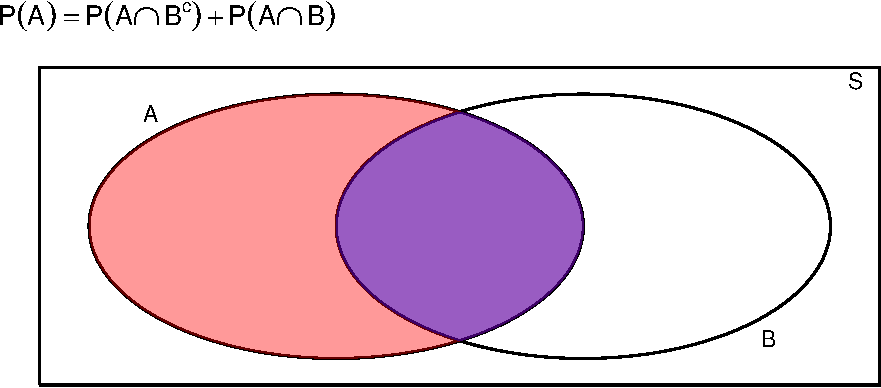
\includegraphics{_main_files/figure-latex/unnamed-chunk-37-1.pdf}

We often want to ask `What is expected value of this distribution?' You
might think about taking a really, really large number of samples from
this distribution and then taking the mean of that really really big
sample. We define the expected value (often denoted by \(\mu\)) as a
weighted average of the possible values and the weights are the
proportions with which those values occur.
\[\mu=E[S]  =   \sum_{\textrm{possible }s}\;s\cdot P\left(S=s\right)\]
In this case, we have that \[\begin{aligned} \mu = E[S] 
&=  \sum_{s=2}^{12}s\cdot P(S=s) \\
&=  2\cdot P\left(S=2\right)+3\cdot P\left(S=3\right)+\dots+11\cdot P\left(S=11\right)+12\cdot P\left(S=12\right) \\
&=  2\left(\frac{1}{36}\right)+3\left(\frac{2}{36}\right)+\dots+11\left(\frac{2}{36}\right)+12\left(\frac{1}{36}\right) \\
&=  7
\end{aligned}\]

\subsubsection{Variance}\label{variance-1}

Similarly we could define the variance of \(S\) (which we often denote
\(\sigma^{2}\)) as a weighted average of the squared-deviations that
could occur.
\[ \sigma^{2}=V[S]  = \sum_{\textrm{possible }s}\; (s-\mu)^2 \cdot P\left(S=s\right)\]
which in this example can be calculated as
\[\begin{aligned} \sigma^{2}=V[S] 
  &= \sum_{s=2}^{12}\left(s-\mu\right)^{2}P(S=s) \\
    &= (2-7)^{2}\left(\frac{1}{36}\right)+(3-7)^{2}\left(\frac{2}{36}\right)+\dots+(12-7)^{2}\left(\frac{1}{36}\right) \\
    &= \frac{35}{6}=5.8\bar{3}
    \end{aligned}\]

We could interpret the expectation as the sample mean of an infinitely
large sample, and the variance as the sample variance of the same
infinitely large sample. These are two very important numbers that
describe the distribution.

\textbf{Example 7}. My wife is a massage therapist and over the last
year, the number of clients she sees per work day (denoted Y ) varied
according the following table:

\begin{longtable}[]{@{}llllll@{}}
\toprule
Number of Clients & 0 & 1 & 2 & 3 & 4\tabularnewline
\midrule
\endhead
\textbf{Frequency/Probability} & 0.30 & 0.35 & 0.20 & 0.10 &
0.05\tabularnewline
\bottomrule
\end{longtable}

\begin{Shaded}
\begin{Highlighting}[]
\NormalTok{distr <-}\StringTok{ }\KeywordTok{data.frame}\NormalTok{(    }\DataTypeTok{clients =} \KeywordTok{c}\NormalTok{( }\DecValTok{0}\NormalTok{,   }\DecValTok{1}\NormalTok{,    }\DecValTok{2}\NormalTok{,    }\DecValTok{3}\NormalTok{,    }\DecValTok{4}   \NormalTok{),    }\CommentTok{# two columns }
                    \DataTypeTok{probability =} \KeywordTok{c}\NormalTok{(}\FloatTok{0.3}\NormalTok{, }\FloatTok{0.35}\NormalTok{, }\FloatTok{0.20}\NormalTok{, }\FloatTok{0.10}\NormalTok{, }\FloatTok{0.05} \NormalTok{) )   }\CommentTok{# }

\KeywordTok{ggplot}\NormalTok{(distr, }\KeywordTok{aes}\NormalTok{(}\DataTypeTok{x=}\NormalTok{clients)) +}\StringTok{                   }\CommentTok{# graph with clients as the x-axis}
\StringTok{  }\KeywordTok{geom_point}\NormalTok{(}\KeywordTok{aes}\NormalTok{(}\DataTypeTok{y=}\NormalTok{probability)) +}\StringTok{                }\CommentTok{# where the dots go}
\StringTok{  }\KeywordTok{geom_linerange}\NormalTok{(}\KeywordTok{aes}\NormalTok{(}\DataTypeTok{ymax=}\NormalTok{probability, }\DataTypeTok{ymin=}\DecValTok{0}\NormalTok{)) +}\StringTok{ }\CommentTok{# the vertical lines       }
\StringTok{  }\KeywordTok{theme_bw}\NormalTok{()                                      }\CommentTok{# set background color...}
\end{Highlighting}
\end{Shaded}

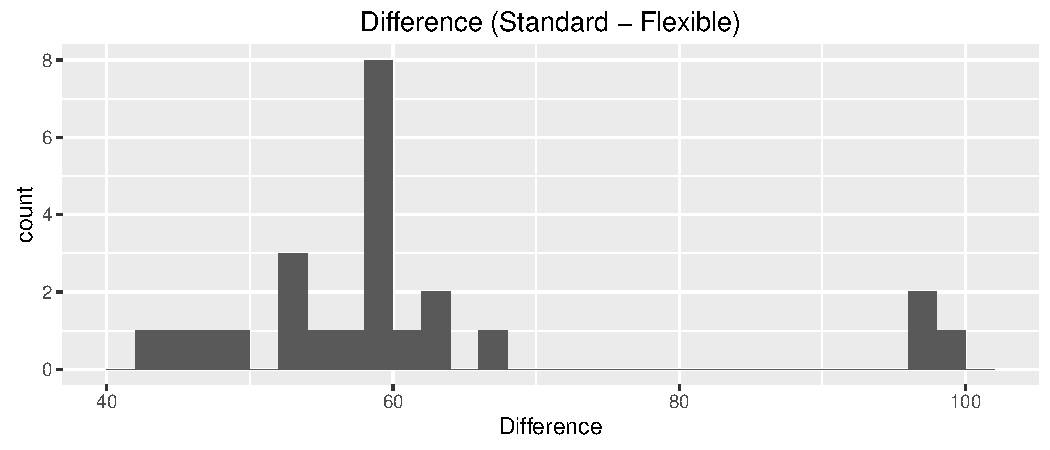
\includegraphics{_main_files/figure-latex/unnamed-chunk-38-1.pdf}
Because this is the long term relative frequency of the number of
clients (over 200 working days!), it is appropriate to interpret these
frequencies as probabilities. This table and graph is often called a
probability mass function (pmf) because it lists how the probability is
spread across the possible values of the random variable. We might next
ask ourselves what is the average number of clients per day? It looks
like it ought to be between 1 and 2 clients per day.
\[\begin{aligned} E\left(Y\right)   
  &=    \sum_{\textrm{possible }y}y\,P\left(Y=y\right) \\
    &=  \sum_{y=0}^{4}y\,P\left(Y=y\right) \\
    &=  0\,P\left(Y=0\right)+1\,P\left(Y=1\right)+2\,P\left(Y=2\right)+3\,P\left(Y=3\right)+4\,P\left(Y=4\right) \\
    &=  0\left(0.3\right)+1\left(0.35\right)+2\left(0.20\right)+3\left(0.10\right)+4\left(0.05\right) \\
    &=  1.25 \end{aligned}\]

Assuming that successive days are independent (which might be a bad
assumption) what is the probability she has two days in a row with no
clients?
\[\begin{aligned}P\left(\textrm{0 on day1 }and\textrm{ 0 on day2}\right)    
  &=    P\left(\textrm{0 on day 1}\right)P\left(\textrm{0 on day 2}\right) \\
    &=  \left(0.3\right)\left(0.3\right) \\
    &=  0.09 \end{aligned}\]

What is the variance of this distribution?
\[\begin{aligned}V\left(Y\right)    
  &= \sum_{\textrm{possible y}}\,\left(y-\mu\right)^{2}\,P\left(Y=y\right) \\
    &= \sum_{y=0}^{4}\,\left(y-\mu\right)^{2}P\left(Y=y\right) \\
    &=  \left(0-1.25\right)^{2}\left(0.3\right)+\left(1-1.25\right)^{2}\left(0.35\right)+\left(2-1.25\right)^{2}\left(0.20\right)+\left(3-1.25\right)^{2}\left(0.10\right)+\left(4-1.25\right)^{2}\left(0.05\right) \\
    &=  1.2875 \end{aligned}\]

Note on Notation: There is a difference between the upper and lower case
letters we have been using to denote a random variable. In general, we
let the upper case denote the random variable and the lower case as a
value that the the variable could possibly take on. So in the massage
example, the number of clients seen per day \(Y\) could take on values
\(y=0,1,2,3,\) or \(4\).

\section{Common Discrete
Distributions}\label{common-discrete-distributions}

\subsection{Binomial Distribution}\label{binomial-distribution}

\textbf{Example}: Suppose we are trapping small mammals in the desert
and we spread out three traps. Assume that the traps are far enough
apart that having one being filled doesn't affect the probability of the
others being filled and that all three traps have the same probability
of being filled in an evening. Denote the event that a trap is filled
with a critter as \(C_{i}\) and denote the event that the trap is empty
as \(E_{i}\). Denote the probability that a trap is filled by \pi=0.8.
(This sort of random variable is often referred to as a Bernoulli RV.)

The possible outcomes are

\begin{longtable}[]{@{}ll@{}}
\toprule
Outcome & \(\,\)\tabularnewline
\midrule
\endhead
\(E_1, E_2, E_3\) & \(\,\)\tabularnewline
\(C_1, E_2, E_3\) & \(\,\)\tabularnewline
\(E_1, C_2, E_3\) & \(\,\)\tabularnewline
\(E_1, E_2, C_3\) & \(\,\)\tabularnewline
\(C_1, C_2, E_3\) & \(\,\)\tabularnewline
\(C_1, E_2, C_3\) & \(\,\)\tabularnewline
\(E_1, C_2, C_3\) & \(\,\)\tabularnewline
\(C_1, C_2, C_3\) & \(\,\)\tabularnewline
\bottomrule
\end{longtable}

Because these are far apart enough in space that the outcome of Trap1 is
independent of Trap2 and Trap3, then
\[P(E_{1}\cap C_{2}\cap E_{3})  =   P(E_{1})P(C_{2})P(E_{3})
    =   (1-0.8)0.8(1-0.8)
    =   0.032\] \textbf{Notice how important the assumption of
independence is!!!} Similarly we could calculate the probabilities for
the rest of the table.

\begin{longtable}[]{@{}llll@{}}
\toprule
Outcome & Probability & \(S\) Outcome & Probability\tabularnewline
\midrule
\endhead
\(E_1, E_2, E_3\) & 0.008 & \(S=0\) & 0.008\tabularnewline
------------------- & --------------- & ------------- &
---------------\tabularnewline
\(C_1, E_2, E_3\) & 0.032 & &\tabularnewline
\(E_1, C_2, E_3\) & 0.032 & \(S=1\) &
\(3(0.032) = 0.096\)\tabularnewline
\(E_1, E_2, C_3\) & 0.032 & &\tabularnewline
------------------- & --------------- & ------------- &
---------------\tabularnewline
\(C_1, C_2, E_3\) & 0.128 & &\tabularnewline
\(C_1, E_2, C_3\) & 0.128 & \(S=2\) &
\(3(0.128) = 0.384\)\tabularnewline
\(E_1, C_2, C_3\) & 0.128 & &\tabularnewline
------------------- & --------------- & ------------- &
---------------\tabularnewline
\(C_1, C_2, C_3\) & 0.512 & \(S=3\) & \(0.512\)\tabularnewline
\bottomrule
\end{longtable}

Next we are interested in the random variable \(S\), the number of traps
that were filled:

\begin{longtable}[]{@{}ll@{}}
\toprule
\(S\) Outcome & Probability\tabularnewline
\midrule
\endhead
\(S=0\) & \(0.008\)\tabularnewline
\(S=1\) & \(0.096\)\tabularnewline
\(S=2\) & \(0.384\)\tabularnewline
\(S=3\) & \(0.512\)\tabularnewline
\bottomrule
\end{longtable}

\(S\) is an example of a Binomial Random Variable. A binomial experiment
is one that:

\begin{enumerate}
\def\labelenumi{\arabic{enumi}.}
\tightlist
\item
  Experiment consists of \(n\) identical trials.
\item
  Each trial results in one of two outcomes (Heads/Tails,
  presence/absence). One will be labeled a success and the other a
  failure.
\item
  The probability of success on a single trial is equal to \(\pi\) and
  remains the same from trial to trial.
\item
  The trials are independent (this is implied from property 3).
\item
  The random variable \(Y\) is the number of successes observed during
  \(n\) trials.
\end{enumerate}

Recall that the probability mass function (pmf) describes how the
probability is spread across the possible outcomes, and in this case, I
can describe this via a nice formula. The pmf of a a binomial random
variable \(X\) taken from \(n\) trials each with probability of success
\(\pi\) is

\[P(X=x)=\underbrace{\frac{n!}{x!(n-x)!}}_{orderings}\;\underbrace{\pi^{x}}_{y\,successes}\;\underbrace{(1-\pi)^{n-x}}_{n-y\,failures}\]

where we define \(n!=n(n-1)\dots(2)(1)\) and further define \(0!=1\).
Often the ordering term is written more compactly as
\[{n \choose x}=\frac{n!}{x!\left(n-x\right)!}\].

For our small mammal example we can create a graph that shows the
binomial distribution with the following R code:

\begin{Shaded}
\begin{Highlighting}[]
\NormalTok{dist <-}\StringTok{ }\KeywordTok{data.frame}\NormalTok{( }\DataTypeTok{x=}\DecValTok{0}\NormalTok{:}\DecValTok{3} \NormalTok{) %>%}\StringTok{ }
\StringTok{  }\KeywordTok{mutate}\NormalTok{(}\DataTypeTok{probability =} \KeywordTok{dbinom}\NormalTok{(x, }\DataTypeTok{size=}\DecValTok{3}\NormalTok{, }\DataTypeTok{prob=}\FloatTok{0.8}\NormalTok{))}
\KeywordTok{ggplot}\NormalTok{(dist, }\KeywordTok{aes}\NormalTok{(}\DataTypeTok{x=}\NormalTok{x)) +}
\StringTok{  }\KeywordTok{geom_point}\NormalTok{(}\KeywordTok{aes}\NormalTok{(}\DataTypeTok{y=}\NormalTok{probability)) +}
\StringTok{  }\KeywordTok{geom_linerange}\NormalTok{(}\KeywordTok{aes}\NormalTok{(}\DataTypeTok{ymax=}\NormalTok{probability, }\DataTypeTok{ymin=}\DecValTok{0}\NormalTok{)) +}
\StringTok{  }\KeywordTok{ggtitle}\NormalTok{(}\StringTok{'Binomial distribution: n=3, p=0.8'}\NormalTok{) +}
\StringTok{  }\KeywordTok{theme_bw}\NormalTok{()}
\end{Highlighting}
\end{Shaded}

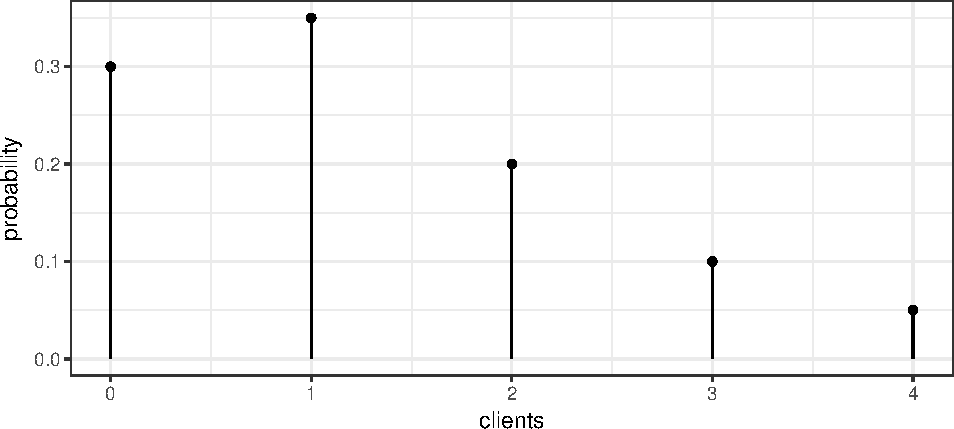
\includegraphics{_main_files/figure-latex/unnamed-chunk-39-1.pdf}

To calculate the height of any of these bars, we can evaluate the pmf at
the desired point. For example, to calculate the probability the number
of full traps is 2, we calculate the following

\[\begin{aligned} P(X=2)    
  &=    {3 \choose 2}\left(0.8\right)^{2}\left(1-0.8\right)^{3-2} \\
    &=  \frac{3!}{2!(3-2)!}(0.8)^{2}(0.2)^{3-2} \\
    &=  \frac{3\cdot2\cdot1}{(2\cdot1)1}\;(0.8)^{2}(0.2) \\
    &=  3(0.128) \\
    &=  0.384 \end{aligned}\]

You can use R to calculate these probabilities. In general, for any
distribution, the ``d-function'' gives the distribution function (pmf or
pdf). So to get R to do the preceding calculation we use:

\begin{Shaded}
\begin{Highlighting}[]
\CommentTok{# If    X ~ Binomial(n=3, pi=0.8)}
\CommentTok{# Then  P( X = 2 | n=3, pi=0.8 ) =}
\KeywordTok{dbinom}\NormalTok{(}\DecValTok{2}\NormalTok{, }\DataTypeTok{size=}\DecValTok{3}\NormalTok{, }\DataTypeTok{prob=}\FloatTok{0.8}\NormalTok{)}
\end{Highlighting}
\end{Shaded}

\begin{verbatim}
## [1] 0.384
\end{verbatim}

The expectation of this distribution can be shown to be
\[\begin{aligned}E[X]   
  &=    \sum_{x=0}^{n}x\,P(X=x) \\
    &=  \sum_{x=0}^{n}x\;\frac{n!}{x!\left(n-x\right)!}\pi^{x}\left(1-\pi\right)^{n-x}\\
    &=  \vdots \\
    &=  n\pi \end{aligned}\]

and the variance can be similarly calculated \[\begin{aligned} V[X]  
  &=    \sum_{x=0}^{n}\left(x-E\left[X\right]\right)^{2}\,P\left(X=x|n,\pi\right) \\
    &=  \sum_{x=0}^{n}\left(x-E\left[X\right]\right)^{2}\;\frac{n!}{x!\left(n-x\right)!}\pi^{x}\left(1-\pi\right)^{n-x} \\
    &=  \vdots \\
    &=  n\pi(1-\pi) \end{aligned}\]

\textbf{Example 8}. Suppose a bird survey only captures the presence or
absence of a particular bird (say the mountain chickadee). Assuming the
true presence proportion at national forest sites around Flagstaff
\[\pi=0.1\], then for \(n=20\) randomly chosen sites, the number of
sites in which the bird was observed would have the distribution

\begin{Shaded}
\begin{Highlighting}[]
\NormalTok{dist <-}\StringTok{ }\KeywordTok{data.frame}\NormalTok{( }\DataTypeTok{x =} \DecValTok{0}\NormalTok{:}\DecValTok{20} \NormalTok{) %>%}\StringTok{ }
\StringTok{  }\KeywordTok{mutate}\NormalTok{(}\DataTypeTok{probability =} \KeywordTok{dbinom}\NormalTok{(x, }\DataTypeTok{size=}\DecValTok{20}\NormalTok{, }\DataTypeTok{prob=}\FloatTok{0.1}\NormalTok{))}
\KeywordTok{ggplot}\NormalTok{(dist, }\KeywordTok{aes}\NormalTok{(}\DataTypeTok{x=}\NormalTok{x)) +}
\StringTok{  }\KeywordTok{geom_point}\NormalTok{(}\KeywordTok{aes}\NormalTok{(}\DataTypeTok{y=}\NormalTok{probability)) +}
\StringTok{  }\KeywordTok{geom_linerange}\NormalTok{(}\KeywordTok{aes}\NormalTok{(}\DataTypeTok{ymax=}\NormalTok{probability, }\DataTypeTok{ymin=}\DecValTok{0}\NormalTok{)) +}
\StringTok{  }\KeywordTok{ggtitle}\NormalTok{(}\StringTok{'Binomial distribution: n=20, p=0.1'}\NormalTok{) +}
\StringTok{  }\KeywordTok{xlab}\NormalTok{(}\StringTok{'Number of Sites Occupied'}\NormalTok{) +}
\StringTok{  }\KeywordTok{theme_bw}\NormalTok{()}
\end{Highlighting}
\end{Shaded}

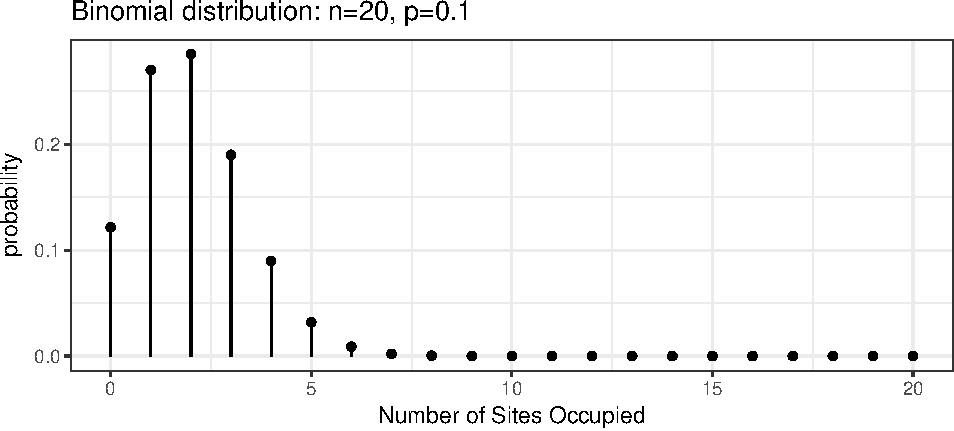
\includegraphics{_main_files/figure-latex/unnamed-chunk-41-1.pdf}

Often we are interested in questions such as \(P(X\le2)\) which is the
probability that we see 2 or fewer of the sites being occupied by
mountain chickadee. These calculations can be tedious to calculate by
hand but R will calculate these cumulative distribution function values
for you using the ``p-function''. This cumulative distribution function
gives the sum of all values up to and including the number given.

\begin{Shaded}
\begin{Highlighting}[]
\CommentTok{# P(X=0) + P(X=1) + P(X=2)}
\NormalTok{sum <-}\StringTok{ }\KeywordTok{dbinom}\NormalTok{(}\DecValTok{0}\NormalTok{, }\DataTypeTok{size=}\DecValTok{20}\NormalTok{, }\DataTypeTok{prob=}\FloatTok{0.1}\NormalTok{) +}\StringTok{ }
\StringTok{       }\KeywordTok{dbinom}\NormalTok{(}\DecValTok{1}\NormalTok{, }\DataTypeTok{size=}\DecValTok{20}\NormalTok{, }\DataTypeTok{prob=}\FloatTok{0.1}\NormalTok{) +}\StringTok{ }
\StringTok{       }\KeywordTok{dbinom}\NormalTok{(}\DecValTok{2}\NormalTok{, }\DataTypeTok{size=}\DecValTok{20}\NormalTok{, }\DataTypeTok{prob=}\FloatTok{0.1}\NormalTok{)}
\NormalTok{sum}
\end{Highlighting}
\end{Shaded}

\begin{verbatim}
## [1] 0.6769268
\end{verbatim}

\begin{Shaded}
\begin{Highlighting}[]
\CommentTok{# P(X <= 2)}
\KeywordTok{pbinom}\NormalTok{(}\DecValTok{2}\NormalTok{, }\DataTypeTok{size=}\DecValTok{20}\NormalTok{, }\DataTypeTok{prob=}\FloatTok{0.1}\NormalTok{)}
\end{Highlighting}
\end{Shaded}

\begin{verbatim}
## [1] 0.6769268
\end{verbatim}

In general we will be interested in asking four different questions
about a distribution.

\begin{enumerate}
\def\labelenumi{\arabic{enumi}.}
\tightlist
\item
  What is the height of the probability mass function (or probability
  density function). For discrete variable \(Y\) this is
  \(P\left(Y=y\right)\) for whatever value of \(y\) we want. In R, this
  will be the \texttt{d}-function.
\item
  What is the probability of observing a value less than or equal to
  \(y\)? In other words, to calculate \(P\left(Y\le y\right)\). In R,
  this will be the \texttt{p}-function.
\item
  What is a particular quantile of a distribution? For example, what
  value separates the lower \(25\%\) from the upper \(75\%\)? In R, this
  will be the \texttt{q}-function.
\item
  Generate a random sample of values from a specified distribution. In
  R, this will be the \texttt{r}-function.
\end{enumerate}

\subsection{Poisson Distribution}\label{poisson-distribution}

A commonly used distribution for count data is the Poisson.

\begin{enumerate}
\def\labelenumi{\arabic{enumi}.}
\tightlist
\item
  Number of customers arriving over a 5 minute interval
\item
  Number of birds observed during a 10 minute listening period
\item
  Number of prairie dog towns per 1000 hectares
\item
  Number of alga clumps per cubic meter of lake water
\end{enumerate}

For a RV is a Poisson RV if the following conditions apply:

\begin{enumerate}
\def\labelenumi{\arabic{enumi}.}
\tightlist
\item
  Two or more events do not occur at precisely the same time or in the
  same space
\item
  The occurrence of an event in a given period of time or region of
  space is independent of the occurrence of the event in a non
  overlapping period or region.
\item
  The expected number of events during one period or region,
  \(\lambda\), is the same in all periods or regions of the same size.
\end{enumerate}

Assuming that these conditions hold for some count variable \(Y\), the
the probability mass function is given by
\[P(Y=y)=\frac{\lambda^{y}e^{-\lambda}}{y!}\] where \(\lambda\) is the
expected number of events over 1 unit of time or space and \(e\) is the
constant \(2.718281828\dots\).

\[E[Y]  =   \lambda\] \[Var[Y]    =   \lambda\]

\textbf{Example 9}. Suppose we are interested in the population size of
small mammals in a region. Let \(Y\) be the number of small mammals
caught in a large trap (multiple traps in the same location?) in a 12
hour period. Finally, suppose that \(Y\sim Poi(\lambda=2.3)\). What is
the probability of finding exactly 4 critters in our trap?
\[P(Y=4)    =   \frac{2.3^{4}\,e^{-2.3}}{4!} =  0.1169\] What about the
probability of finding at most 4? \[\begin{aligned} P(Y\le4) 
  &=    P(Y=0)+P(Y=1)+P(Y=2)+P(Y=3)+P(Y=4) \\
    &=  0.1003+0.2306+0.2652+0.2033+0.1169 \\
    &=  0.9163 \end{aligned}\]

What about the probability of finding 5 or more?
\[P(Y\ge5)  =   1-P(Y\le4) =    1-0.9163 =  0.0837\]

These calculations can be done using the distribution function
(d-function) for the poisson and the cumulative distribution function
(p-function).

\begin{Shaded}
\begin{Highlighting}[]
\NormalTok{dist <-}\StringTok{ }\KeywordTok{data.frame}\NormalTok{( }\DataTypeTok{NumCaught =} \DecValTok{0}\NormalTok{:}\DecValTok{10} \NormalTok{) %>%}
\StringTok{  }\KeywordTok{mutate}\NormalTok{( }\DataTypeTok{probability =} \KeywordTok{dpois}\NormalTok{( NumCaught, }\DataTypeTok{lambda=}\FloatTok{2.3} \NormalTok{) )}
\KeywordTok{ggplot}\NormalTok{(dist, }\KeywordTok{aes}\NormalTok{(}\DataTypeTok{x=}\NormalTok{NumCaught)) +}
\StringTok{  }\KeywordTok{geom_point}\NormalTok{( }\KeywordTok{aes}\NormalTok{(}\DataTypeTok{y=}\NormalTok{probability) ) +}
\StringTok{  }\KeywordTok{geom_linerange}\NormalTok{(}\KeywordTok{aes}\NormalTok{( }\DataTypeTok{ymax=}\NormalTok{probability, }\DataTypeTok{ymin=}\DecValTok{0}\NormalTok{)) +}
\StringTok{  }\KeywordTok{ggtitle}\NormalTok{(}\KeywordTok{expression}\NormalTok{(}\KeywordTok{paste}\NormalTok{(}\StringTok{'Poisson Distribution with  '}\NormalTok{, lambda ==}\StringTok{ }\FloatTok{2.3}\NormalTok{))) +}
\StringTok{  }\KeywordTok{labs}\NormalTok{(}\DataTypeTok{x=}\StringTok{'Number Caught'}\NormalTok{) +}
\StringTok{  }\KeywordTok{theme_bw}\NormalTok{()            }
\end{Highlighting}
\end{Shaded}

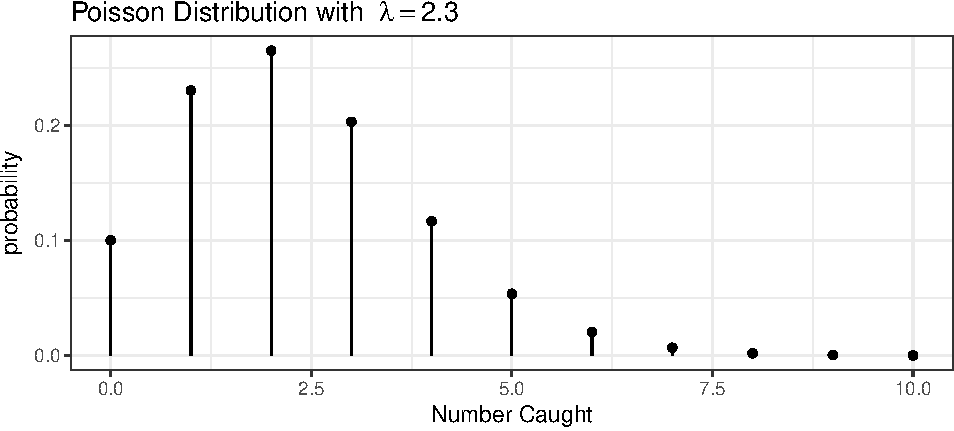
\includegraphics{_main_files/figure-latex/unnamed-chunk-43-1.pdf}

\begin{Shaded}
\begin{Highlighting}[]
\CommentTok{# P( Y = 4)}
\KeywordTok{dpois}\NormalTok{(}\DecValTok{4}\NormalTok{, }\DataTypeTok{lambda=}\FloatTok{2.3}\NormalTok{)}
\end{Highlighting}
\end{Shaded}

\begin{verbatim}
## [1] 0.1169022
\end{verbatim}

\begin{Shaded}
\begin{Highlighting}[]
\CommentTok{# P( Y <= 4)}
\KeywordTok{ppois}\NormalTok{(}\DecValTok{4}\NormalTok{, }\DataTypeTok{lambda=}\FloatTok{2.3}\NormalTok{)}
\end{Highlighting}
\end{Shaded}

\begin{verbatim}
## [1] 0.9162493
\end{verbatim}

\begin{Shaded}
\begin{Highlighting}[]
\CommentTok{# 1-P(Y <= 4)  ==  P( Y > 4)  ==  P( Y >= 5)}
\DecValTok{1}\NormalTok{-}\KeywordTok{ppois}\NormalTok{(}\DecValTok{4}\NormalTok{, }\FloatTok{2.3}\NormalTok{)}
\end{Highlighting}
\end{Shaded}

\begin{verbatim}
## [1] 0.08375072
\end{verbatim}

\section{Continuous Random Variables}\label{continuous-random-variables}

Continuous random variables can take on an (uncountably) infinite number
of values, and this results in a few obnoxious mathematical differences
between how we handle continuous and discrete random variables. In
particular, the probability that a continuous random variable \(X\) will
take on a particular value will be zero, so we will be interested in
finding the probability that the random variable is in some interval
instead. Wherever we had a summation, \(\sum\), we will instead have an
integral, but because many students haven't had calculus, we will resort
to using R or tables of calculated values.

\subsection{Uniform(0,1) Distribution}\label{uniform01-distribution}

Suppose you wish to draw a random number number between 0 and 1 and any
two intervals of equal size should have the same probability of the
value being in them. This random variable is said to have a Uniform(0,1)
distribution.

Because there are an infinite number of rational numbers between 0 and
1, the probability of any particular number being selected is
\(1/\infty=0\). But even though each number has 0 probability of being
selected, some number must end up being selected. Because of this
conundrum, probability theory doesn't look at the probability of a
single number, but rather focuses on a region of numbers.

To make this distinction, we will define the distribution using a
probability density function (pdf) instead of the probability mass
function. In the discrete case, we had to constrain the probability mass
function to sum to 1. In the continuous case, we have to constrain the
probability density function to integrate to 1.

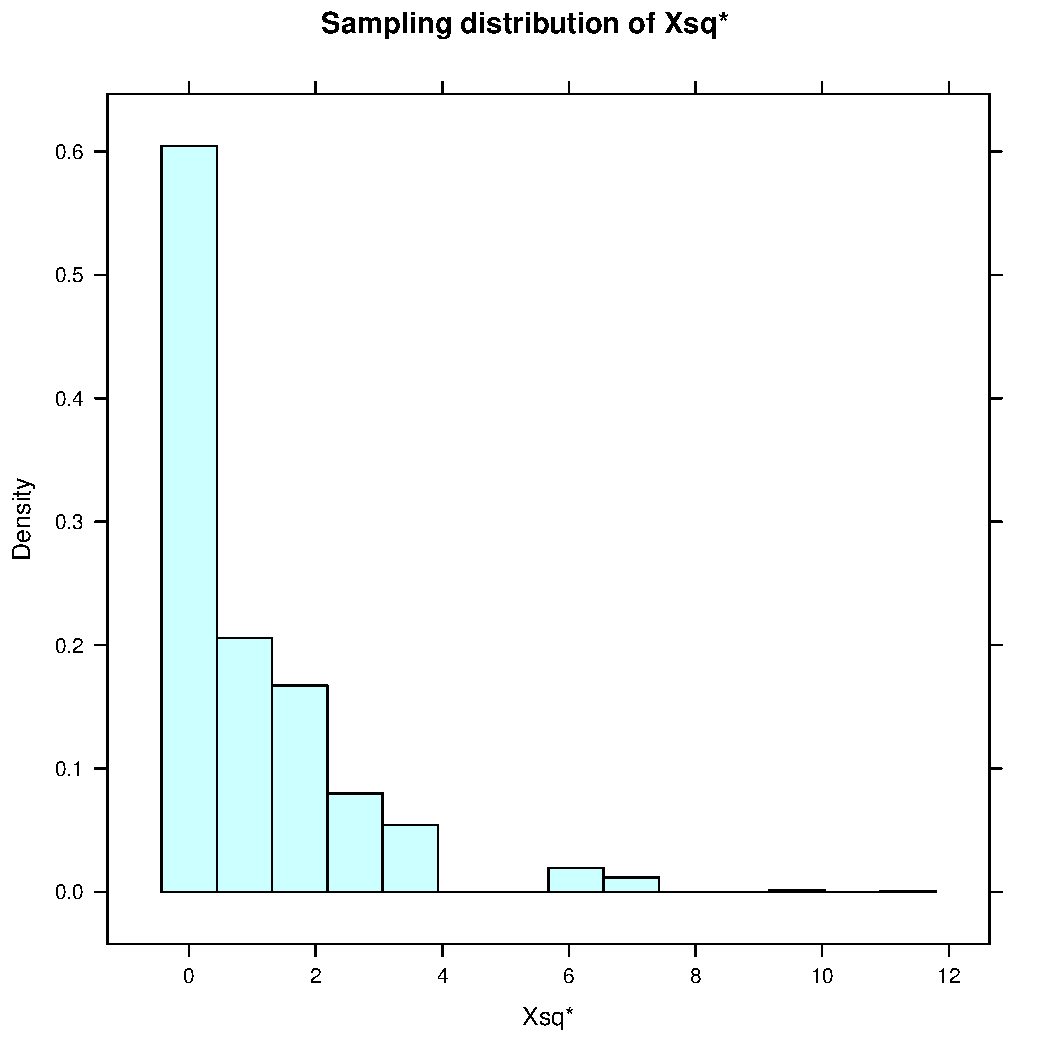
\includegraphics{_main_files/figure-latex/unnamed-chunk-44-1.pdf}

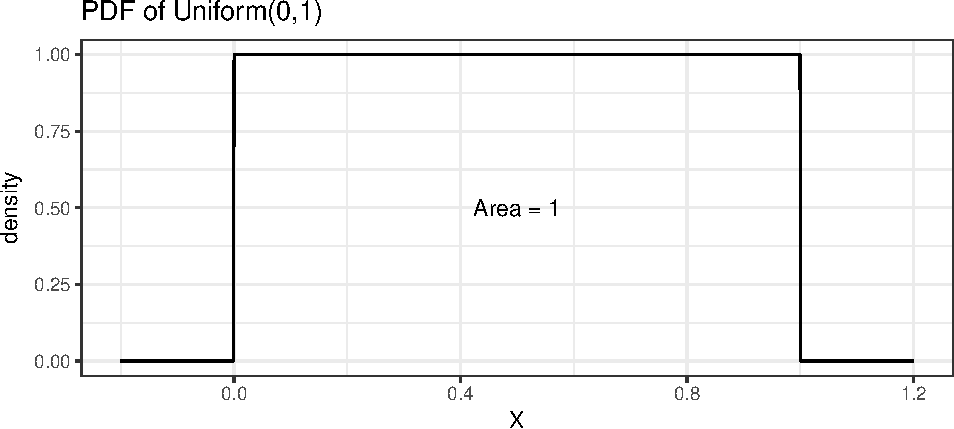
\includegraphics{_main_files/figure-latex/unnamed-chunk-45-1.pdf}

Finding the area under the curve of a particular density function
\(f(x)\) usually requires the use of calculus, but since this isn't a
calculus course, we will resort to using R or tables of calculated
values.

\subsection{Exponential Distribution}\label{exponential-distribution}

The exponential distribution is the continuous analog of the Poisson
distribution and is often used to model the time between occurrence of
successive events. Perhaps we are modeling time between transmissions on
a network, or the time between feeding events or prey capture. If the
random variable \(X\) has an Exponential distribution, its probability
density function is \[f(x)=\begin{cases}
\lambda e^{-\lambda x} & x\ge0\;\textrm{ and }\;\lambda>0\\
0 & \textrm{otherwise}
\end{cases}\]

Analogous to the discrete distributions, we can define the Expectation
and Variance of these distributions by replacing the summation with an
integral
\[\mu = E[X] =  \int_{0}^{\infty}x\,f(x)\,dx = \dots = \frac{1}{\lambda} \]
\[\sigma^2 = Var[X] =   \int_{0}^{\infty}\left(x-\mu\right)^{2}\,f\left(x\right)\,dx =  \dots = \frac{1}{\lambda^{2}}\]

Because the exponential distribution is defined by the rate of
occurrence of an event, increasing that rate decreases the time between
events. Furthermore because the rate of occurrence cannot be negative,
we restrict \(\lambda>0\).

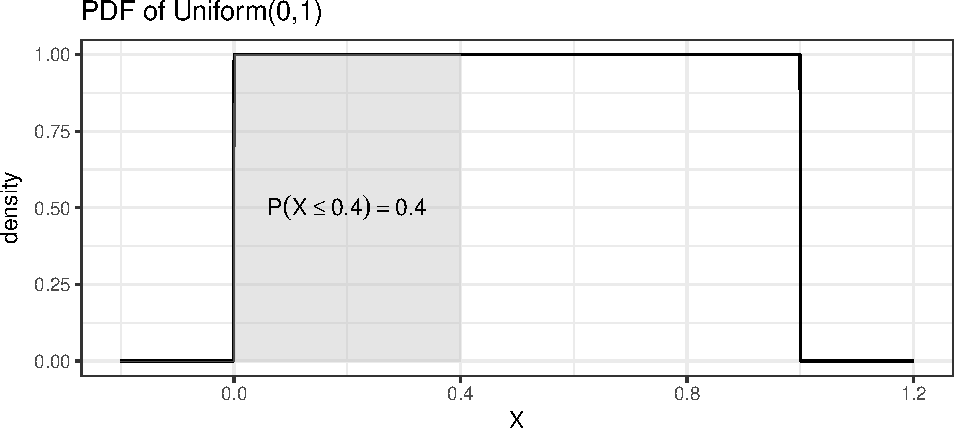
\includegraphics{_main_files/figure-latex/unnamed-chunk-46-1.pdf}

\textbf{Example 10}. Suppose the time between insect captures \(X\)
during a summer evening for a species of bat follows a exponential
distribution with capture rate of \(\lambda=2\) insects per minute and
therefore the expected waiting time between captures is
\(1/\lambda=1/2\) minute. Suppose that we are interested in the
probability that it takes a bat more than 1 minute to capture its next
insect.

\[P(X>1)=\]

\begin{Shaded}
\begin{Highlighting}[]
\NormalTok{data <-}\StringTok{ }\KeywordTok{data.frame}\NormalTok{(}\DataTypeTok{x=}\KeywordTok{seq}\NormalTok{(}\DecValTok{0}\NormalTok{,}\DecValTok{5}\NormalTok{,}\DataTypeTok{length=}\DecValTok{1000}\NormalTok{), }\DataTypeTok{lambda =} \DecValTok{2}\NormalTok{) %>%}
\StringTok{  }\KeywordTok{mutate}\NormalTok{(}\DataTypeTok{y=}\KeywordTok{dexp}\NormalTok{(x, }\DataTypeTok{rate =} \NormalTok{lambda),}
         \DataTypeTok{grp =} \KeywordTok{ifelse}\NormalTok{( x >}\StringTok{ }\DecValTok{1}\NormalTok{, }\StringTok{'> 1'}\NormalTok{, }\StringTok{'<= 1'}\NormalTok{))}
\KeywordTok{ggplot}\NormalTok{(data, }\KeywordTok{aes}\NormalTok{(}\DataTypeTok{x=}\NormalTok{x, }\DataTypeTok{y=}\NormalTok{y, }\DataTypeTok{fill=}\NormalTok{grp)) +}
\StringTok{  }\KeywordTok{geom_area}\NormalTok{() +}
\StringTok{  }\KeywordTok{labs}\NormalTok{(}\DataTypeTok{y=}\StringTok{'density'}\NormalTok{) +}
\StringTok{  }\KeywordTok{theme_bw}\NormalTok{()}
\end{Highlighting}
\end{Shaded}

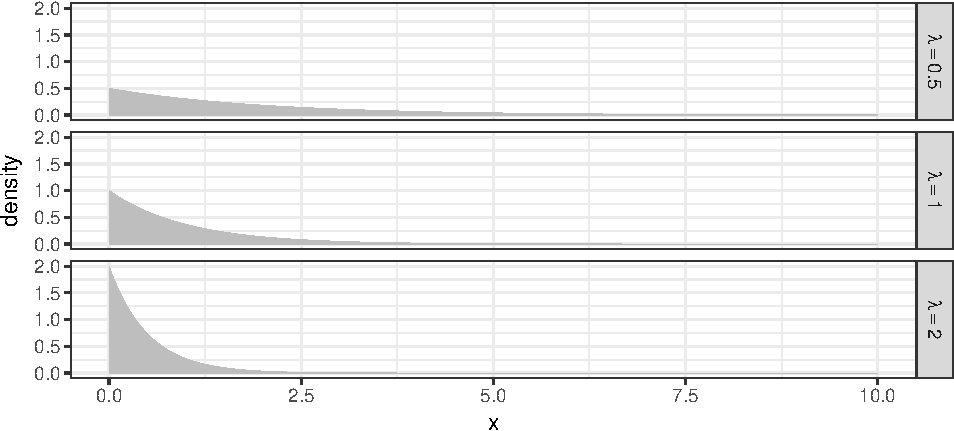
\includegraphics{_main_files/figure-latex/unnamed-chunk-47-1.pdf}

We now must resort to calculus to find this area. Or use tables of
pre-calculated values. Or use R, remembering that p-functions give the
area under the curve to the left of the given value.

\begin{Shaded}
\begin{Highlighting}[]
\CommentTok{# P(X > 1)  == 1 - P(X <= 1)}
\DecValTok{1} \NormalTok{-}\StringTok{ }\KeywordTok{pexp}\NormalTok{(}\DecValTok{1}\NormalTok{, }\DataTypeTok{rate=}\DecValTok{2}\NormalTok{)}
\end{Highlighting}
\end{Shaded}

\begin{verbatim}
## [1] 0.1353353
\end{verbatim}

\subsection{Normal Distribution}\label{normal-distribution}

Undoubtably the most important distribution in statistics is the normal
distribution. If my RV \(X\) is normally distributed with mean \(\mu\)
and standard deviation \(\sigma\), its probability density function is
given by
\[f(x)=\frac{1}{\sqrt{2\pi}\sigma}\exp\left[\frac{-(x-\mu)^{2}}{2\sigma^{2}}\right]\]
where \(\exp[y]\) is the exponential function \(e^{y}\). We could
slightly rearrange the function to

\[f(x)=\frac{1}{\sqrt{2\pi}\sigma}\exp\left[-\frac{1}{2}\left(\frac{x-\mu}{\sigma}\right)^{2}\right]\]

and see this distribution is defined by its expectation \(E[X]=\mu\) and
its variance \(Var[X]=\sigma^{2}\). Notice I could define it using the
standard deviation \(\sigma\), and different software packages will
expect it to be defined by one or the other. R defines the normal
distribution using the standard deviation.

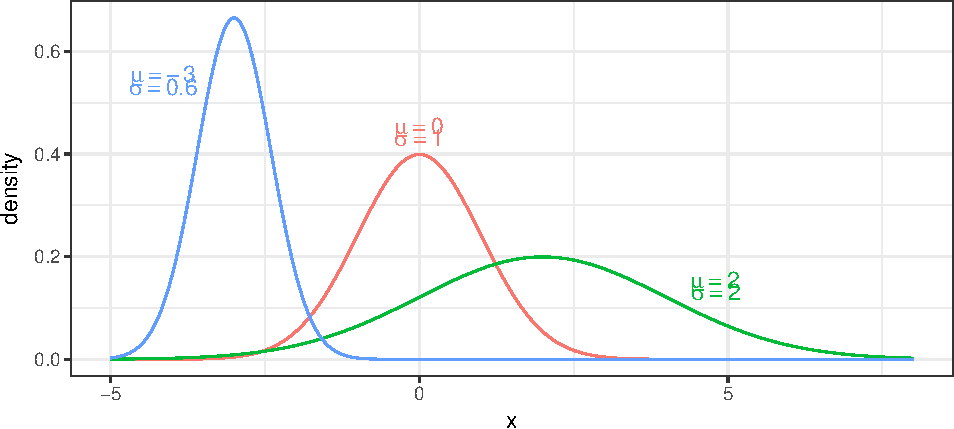
\includegraphics{_main_files/figure-latex/unnamed-chunk-49-1.pdf}

\textbf{Example 11}. It is known that the heights of adult males in the
US is approximately normal with a mean of 5 feet 10 inches (\(\mu=70\)
inches) and a standard deviation of \(\sigma=3\) inches. Your instructor
is a mere 5 feet 4 inches (64 inches). What proportion of the population
is shorter than your professor?

\begin{Shaded}
\begin{Highlighting}[]
\NormalTok{distr <-}\StringTok{ }\KeywordTok{data.frame}\NormalTok{(}\DataTypeTok{x=}\KeywordTok{seq}\NormalTok{(}\DecValTok{57}\NormalTok{, }\DecValTok{82}\NormalTok{, }\DataTypeTok{length=}\DecValTok{1000}\NormalTok{)) %>%}
\StringTok{  }\KeywordTok{mutate}\NormalTok{( }\DataTypeTok{density =} \KeywordTok{dnorm}\NormalTok{(x, }\DataTypeTok{mean=}\DecValTok{70}\NormalTok{, }\DataTypeTok{sd=}\DecValTok{3}\NormalTok{),}
          \DataTypeTok{group =} \KeywordTok{ifelse}\NormalTok{(x<=}\DecValTok{64}\NormalTok{, }\StringTok{'Shorter'}\NormalTok{,}\StringTok{'Taller'}\NormalTok{) )}
\KeywordTok{ggplot}\NormalTok{(distr, }\KeywordTok{aes}\NormalTok{(}\DataTypeTok{x=}\NormalTok{x, }\DataTypeTok{y=}\NormalTok{density, }\DataTypeTok{fill=}\NormalTok{group)) +}
\StringTok{  }\KeywordTok{geom_line}\NormalTok{() +}
\StringTok{  }\KeywordTok{geom_area}\NormalTok{() +}
\StringTok{  }\KeywordTok{theme_bw}\NormalTok{()}
\end{Highlighting}
\end{Shaded}

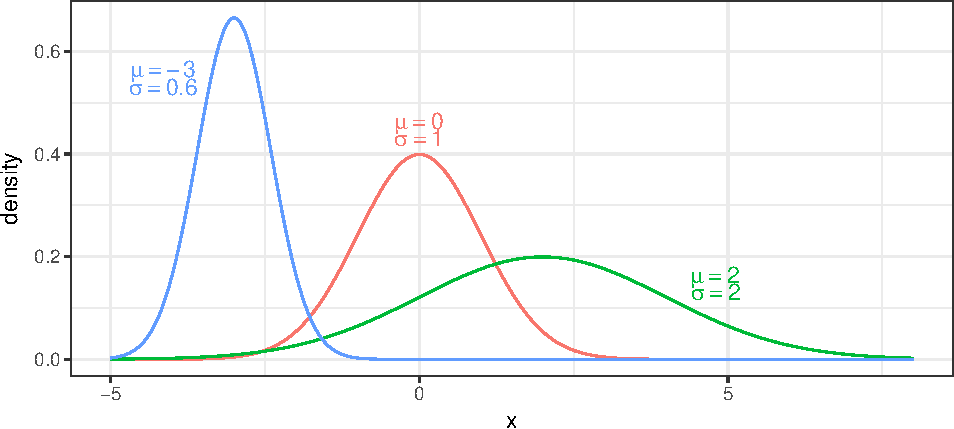
\includegraphics{_main_files/figure-latex/unnamed-chunk-50-1.pdf}

Using R you can easily find this

\begin{Shaded}
\begin{Highlighting}[]
\KeywordTok{pnorm}\NormalTok{(}\DecValTok{64}\NormalTok{, }\DataTypeTok{mean=}\DecValTok{70}\NormalTok{, }\DataTypeTok{sd=}\DecValTok{3}\NormalTok{)}
\end{Highlighting}
\end{Shaded}

\begin{verbatim}
## [1] 0.02275013
\end{verbatim}

\subsection{Standardizing}\label{standardizing}

Before we had computers that could calculate these probabilities for any
normal distribution, it was important to know how to convert a
probability statement from an arbitrary \(N\left(\mu,\sigma^{2}\right)\)
distribution to a question about a Stanard Normal distribution, which is
a normal distribution with mean \(\mu=0\) and standard deviation
\(\sigma=1\). If we have \[X\sim N\left(\mu,\sigma^{2}\right)\] then
\[Z=\frac{X-\mu}{\sigma}\sim N\left(0,1\right)\]

You might remember doing something similar in an undergraduate
statistics course in order to use a table to look up some probability.
From the height example, we calculate \[\begin{aligned}z  
  &=    \frac{64-70}{3} \\
    &=  \frac{-6}{3} \\
    &=  -2 \end{aligned}\] Note that this calculation shows that he is
\(-2\) standard deviations from the mean. Next we look at a table for
\(z=-2.00\). To do this we go down to the \(-2.0\) row and over to the
\(.00\) column and find \(0.0228\). Only slightly over 2\% of the adult
male population is shorter!

How tall must a person be to be taller than \(80\%\) of the rest of the
adult male population? To answer that we must use the table in reverse
and look for the \(0.8\) value. We find the closest value possible
\((0.7995)\) and the \(z\) value associated with it is \(z=0.84\). Next
we solve the standardizing equation for \(x\) \[\begin{aligned}
z       &=  \frac{x-\mu}{\sigma} \\
0.84    &=  \frac{x-70}{3} \\
x       &=  3(0.84)+70 \\
        &=  72.49\;\textrm{inches} \end{aligned}\]

Alternatively we could use the quantile function for the normal
distribution (q-function) in R and avoid the imprecision of using a
table.

\begin{Shaded}
\begin{Highlighting}[]
\KeywordTok{qnorm}\NormalTok{(.}\DecValTok{8}\NormalTok{, }\DataTypeTok{mean=}\DecValTok{0}\NormalTok{, }\DataTypeTok{sd=}\DecValTok{1}\NormalTok{)}
\end{Highlighting}
\end{Shaded}

\begin{verbatim}
## [1] 0.8416212
\end{verbatim}

\textbf{Empirical Rule} - It is from the normal distribution that the
empirical rule from the previous chapter is derived. If
\(X\sim N(\mu,\sigma^{2})\) then
\[\begin{aligned} P(\mu-\sigma\le X\le\mu+\sigma)   
  &=    P(-1 \le Z \le 1) \\
    &=  P(Z \le 1) - P(Z \le -1) \\
    &\approx    0.8413-0.1587 \\
    &=  0.6826 \end{aligned}\]

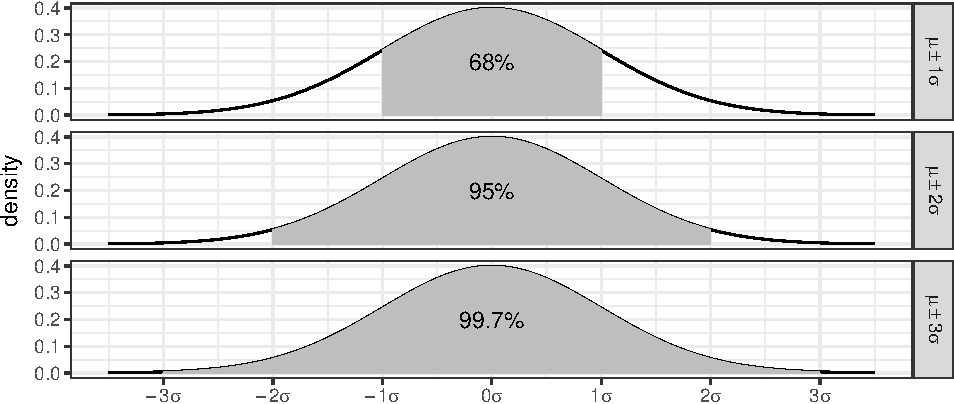
\includegraphics{_main_files/figure-latex/unnamed-chunk-53-1.pdf}

1.6 R Comments

There will be a variety of distributions we'll be interested in and R
refers to them using the following abbreviations

\begin{longtable}[]{@{}llll@{}}
\toprule
\begin{minipage}[b]{0.16\columnwidth}\raggedright\strut
Distribution\strut
\end{minipage} & \begin{minipage}[b]{0.15\columnwidth}\raggedright\strut
Stem\strut
\end{minipage} & \begin{minipage}[b]{0.17\columnwidth}\raggedright\strut
Parameters\strut
\end{minipage} & \begin{minipage}[b]{0.40\columnwidth}\raggedright\strut
Parameter Interpretation\strut
\end{minipage}\tabularnewline
\midrule
\endhead
\begin{minipage}[t]{0.16\columnwidth}\raggedright\strut
Binomial\strut
\end{minipage} & \begin{minipage}[t]{0.15\columnwidth}\raggedright\strut
\texttt{binom}\strut
\end{minipage} & \begin{minipage}[t]{0.17\columnwidth}\raggedright\strut
\texttt{size} \texttt{prob}\strut
\end{minipage} & \begin{minipage}[t]{0.40\columnwidth}\raggedright\strut
Number of Trials Probability of Success (per Trial)\strut
\end{minipage}\tabularnewline
\begin{minipage}[t]{0.16\columnwidth}\raggedright\strut
Exponential\strut
\end{minipage} & \begin{minipage}[t]{0.15\columnwidth}\raggedright\strut
\texttt{exp}\strut
\end{minipage} & \begin{minipage}[t]{0.17\columnwidth}\raggedright\strut
\texttt{rate}\strut
\end{minipage} & \begin{minipage}[t]{0.40\columnwidth}\raggedright\strut
Mean of the distribution\strut
\end{minipage}\tabularnewline
\begin{minipage}[t]{0.16\columnwidth}\raggedright\strut
Normal\strut
\end{minipage} & \begin{minipage}[t]{0.15\columnwidth}\raggedright\strut
\texttt{norm}\strut
\end{minipage} & \begin{minipage}[t]{0.17\columnwidth}\raggedright\strut
\texttt{mean=0} \texttt{sd=1}\strut
\end{minipage} & \begin{minipage}[t]{0.40\columnwidth}\raggedright\strut
Center of the distribution Standard deviation\strut
\end{minipage}\tabularnewline
\begin{minipage}[t]{0.16\columnwidth}\raggedright\strut
Uniform\strut
\end{minipage} & \begin{minipage}[t]{0.15\columnwidth}\raggedright\strut
\texttt{unif}\strut
\end{minipage} & \begin{minipage}[t]{0.17\columnwidth}\raggedright\strut
\texttt{min=0} \texttt{max=1}\strut
\end{minipage} & \begin{minipage}[t]{0.40\columnwidth}\raggedright\strut
Minimum of the distribution Maximum of the distribution\strut
\end{minipage}\tabularnewline
\bottomrule
\end{longtable}

All the probability distributions available in R are accessed in exactly
the same way, using a d-function, p-function, q-function, and
r-function.

\begin{longtable}[]{@{}ll@{}}
\toprule
\begin{minipage}[b]{0.24\columnwidth}\raggedright\strut
Function\strut
\end{minipage} & \begin{minipage}[b]{0.70\columnwidth}\raggedright\strut
Result\strut
\end{minipage}\tabularnewline
\midrule
\endhead
\begin{minipage}[t]{0.24\columnwidth}\raggedright\strut
\texttt{d}-function(x)\strut
\end{minipage} & \begin{minipage}[t]{0.70\columnwidth}\raggedright\strut
The height of the probability distribution/density at \(x\)\strut
\end{minipage}\tabularnewline
\begin{minipage}[t]{0.24\columnwidth}\raggedright\strut
\texttt{p}-function(x)\strut
\end{minipage} & \begin{minipage}[t]{0.70\columnwidth}\raggedright\strut
\(P\left(X\le x\right)\)\strut
\end{minipage}\tabularnewline
\begin{minipage}[t]{0.24\columnwidth}\raggedright\strut
\texttt{q}-function(q)\strut
\end{minipage} & \begin{minipage}[t]{0.70\columnwidth}\raggedright\strut
\(x\) such that \(P\left(X\le x\right) = q\)\strut
\end{minipage}\tabularnewline
\begin{minipage}[t]{0.24\columnwidth}\raggedright\strut
\texttt{r}-function(n)\strut
\end{minipage} & \begin{minipage}[t]{0.70\columnwidth}\raggedright\strut
\(n\) random observations from the distribution\strut
\end{minipage}\tabularnewline
\bottomrule
\end{longtable}

1.7 Exercises

\begin{enumerate}
\def\labelenumi{\arabic{enumi}.}
\item
  The population distribution of blood donors in the United States based
  on race/ethnicity and blood type as reported by the American Red Cross
  is given here:

  \begin{longtable}[]{@{}llllll@{}}
  \toprule
  \begin{minipage}[b]{0.15\columnwidth}\raggedright\strut
  \(\,\)\strut
  \end{minipage} &
  \begin{minipage}[b]{0.10\columnwidth}\raggedright\strut
  O\strut
  \end{minipage} &
  \begin{minipage}[b]{0.12\columnwidth}\raggedright\strut
  A\strut
  \end{minipage} &
  \begin{minipage}[b]{0.10\columnwidth}\raggedright\strut
  B\strut
  \end{minipage} &
  \begin{minipage}[b]{0.10\columnwidth}\raggedright\strut
  AB\strut
  \end{minipage} &
  \begin{minipage}[b]{0.10\columnwidth}\raggedright\strut
  Total\strut
  \end{minipage}\tabularnewline
  \midrule
  \endhead
  \begin{minipage}[t]{0.15\columnwidth}\raggedright\strut
  \textbf{White}\strut
  \end{minipage} &
  \begin{minipage}[t]{0.10\columnwidth}\raggedright\strut
  36\%\strut
  \end{minipage} &
  \begin{minipage}[t]{0.12\columnwidth}\raggedright\strut
  32.2\%\strut
  \end{minipage} &
  \begin{minipage}[t]{0.10\columnwidth}\raggedright\strut
  8.8\%\strut
  \end{minipage} &
  \begin{minipage}[t]{0.10\columnwidth}\raggedright\strut
  3.2\%\strut
  \end{minipage} &
  \begin{minipage}[t]{0.10\columnwidth}\raggedright\strut
  \(\,\)\strut
  \end{minipage}\tabularnewline
  \begin{minipage}[t]{0.15\columnwidth}\raggedright\strut
  \textbf{Black}\strut
  \end{minipage} &
  \begin{minipage}[t]{0.10\columnwidth}\raggedright\strut
  7\%\strut
  \end{minipage} &
  \begin{minipage}[t]{0.12\columnwidth}\raggedright\strut
  2.9\%\strut
  \end{minipage} &
  \begin{minipage}[t]{0.10\columnwidth}\raggedright\strut
  2.5\%\strut
  \end{minipage} &
  \begin{minipage}[t]{0.10\columnwidth}\raggedright\strut
  0.5\%\strut
  \end{minipage} &
  \begin{minipage}[t]{0.10\columnwidth}\raggedright\strut
  \(\,\)\strut
  \end{minipage}\tabularnewline
  \begin{minipage}[t]{0.15\columnwidth}\raggedright\strut
  \textbf{Asian}\strut
  \end{minipage} &
  \begin{minipage}[t]{0.10\columnwidth}\raggedright\strut
  1.7\%\strut
  \end{minipage} &
  \begin{minipage}[t]{0.12\columnwidth}\raggedright\strut
  1.2\%\strut
  \end{minipage} &
  \begin{minipage}[t]{0.10\columnwidth}\raggedright\strut
  1\%\strut
  \end{minipage} &
  \begin{minipage}[t]{0.10\columnwidth}\raggedright\strut
  0.3\%\strut
  \end{minipage} &
  \begin{minipage}[t]{0.10\columnwidth}\raggedright\strut
  \(\,\)\strut
  \end{minipage}\tabularnewline
  \begin{minipage}[t]{0.15\columnwidth}\raggedright\strut
  \textbf{Other}\strut
  \end{minipage} &
  \begin{minipage}[t]{0.10\columnwidth}\raggedright\strut
  1.5\%\strut
  \end{minipage} &
  \begin{minipage}[t]{0.12\columnwidth}\raggedright\strut
  0.8\%\strut
  \end{minipage} &
  \begin{minipage}[t]{0.10\columnwidth}\raggedright\strut
  0.3\%\strut
  \end{minipage} &
  \begin{minipage}[t]{0.10\columnwidth}\raggedright\strut
  0.1\%\strut
  \end{minipage} &
  \begin{minipage}[t]{0.10\columnwidth}\raggedright\strut
  \(\,\)\strut
  \end{minipage}\tabularnewline
  \begin{minipage}[t]{0.15\columnwidth}\raggedright\strut
  \(\,\)\strut
  \end{minipage} &
  \begin{minipage}[t]{0.10\columnwidth}\raggedright\strut
  \(\,\)\strut
  \end{minipage} &
  \begin{minipage}[t]{0.12\columnwidth}\raggedright\strut
  \(\,\)\strut
  \end{minipage} &
  \begin{minipage}[t]{0.10\columnwidth}\raggedright\strut
  \(\,\)\strut
  \end{minipage} &
  \begin{minipage}[t]{0.10\columnwidth}\raggedright\strut
  \(\,\)\strut
  \end{minipage} &
  \begin{minipage}[t]{0.10\columnwidth}\raggedright\strut
  100\%\strut
  \end{minipage}\tabularnewline
  \bottomrule
  \end{longtable}

  Notice that the numbers given in the table sum to 100\%, so the data
  presented are the probability of a particular ethnicity and blood
  type.

  \begin{enumerate}
  \def\labelenumii{\alph{enumii})}
  \tightlist
  \item
    Fill in the column and row totals.
  \item
    What is the probability that a randomly selected donor will be Asian
    and have Type O blood? That is to say, given a donor is randomly
    selected from the list of all donors, what is the probability that
    the selected donor will Asian with Type O?
  \item
    What is the probability that a randomly selected donor is white?
    That is to say, given a donor is randomly selected from the list of
    all donors, what is the probability that the selected donor is
    white?
  \item
    What is the probability that a randomly selected donor has Type A
    blood? That is to say, given a donor is selected from the list of
    all donors, what is the probability that the selected donor has Type
    A blood?
  \item
    What is the probability that a white donor will have Type A blood?
    That is to say, given a donor is randomly selected from the list of
    all the white donors, what is the probability that the selected
    donor has Type A blood? (Notice we already know the donor is white
    because we restricted ourselves to that subset!)
  \item
    Is blood type and ethnicity independent? Justify your response
    mathematically using your responses from the previous answers.
  \end{enumerate}
\item
  For each of the following, mark if it is Continuous or Discrete.

  \begin{enumerate}
  \def\labelenumii{\alph{enumii})}
  \tightlist
  \item
    \(\underline{\hspace{1in}}\) Milliliters of tea drunk per day.
  \item
    \(\underline{\hspace{1in}}\) Different brands of soda drunk over the
    course of a year.
  \item
    \(\underline{\hspace{1in}}\) Number of days per week that you are
    on-campus for any amount of time.
  \item
    \(\underline{\hspace{1in}}\) Number of grizzly bears individuals
    genetically identified from a grid of hair traps in Glacier National
    Park.
  \end{enumerate}
\item
  For each scenario, state whether the event should be modeled via a
  binomial or Poisson distribution.

  \begin{enumerate}
  \def\labelenumii{\alph{enumii})}
  \tightlist
  \item
    \(\underline{\hspace{1in}}\) Number of M\&Ms I eat per hour while
    grading homework
  \item
    \(\underline{\hspace{1in}}\) The number of mornings in the coming 7
    days that I change my son's first diaper of the day.
  \item
    \(\underline{\hspace{1in}}\) The number of Manzanita bushes per 100
    meters of trail.
  \end{enumerate}
\item
  During a road bike race, there is always a chance a crash will occur.
  Suppose the probability that at least one crash will occur in any race
  I'm in is \(\pi=0.2\) and that races are independent.

  \begin{enumerate}
  \def\labelenumii{\alph{enumii})}
  \tightlist
  \item
    What is the probability that the next two races I'm in will both
    have crashes?
  \item
    What is the probability that neither of my next two races will have
    a crash?
  \item
    What is the probability that at least one of the next two races have
    a crash?
  \end{enumerate}
\item
  My cats suffer from gastric distress due to eating house plants and
  the number of vomits per week that I have to clean up follows a
  Poisson distribution with rate \(\lambda=1.2\) pukes per week.

  \begin{enumerate}
  \def\labelenumii{\alph{enumii})}
  \tightlist
  \item
    What is the probability that I don't have to clean up any vomits
    this coming week?
  \item
    What is the probability that I must clean up 1 or more vomits?
  \item
    If I wanted to measure this process with a rate per day, what rate
    should I use?
  \end{enumerate}
\item
  Suppose that the number of runners I see on a morning walk on the
  trails near my house has the following distribution (Notice I've never
  seen four or more runners on a morning walk):

  \begin{longtable}[]{@{}llllll@{}}
  \toprule
  y & 0 & 1 & 2 & 3 & 4+\tabularnewline
  \midrule
  \endhead
  \textbf{Probabilty} & 0.45 & 0.25 & 0.20 & & 0.0\tabularnewline
  \bottomrule
  \end{longtable}

  \begin{enumerate}
  \def\labelenumii{\alph{enumii})}
  \tightlist
  \item
    What is the probability that I see 3 runners on a morning walk?
  \item
    What is the expected number of runners that I will encounter?
  \item
    What is the variance of the number of runners that I will encounter?
  \end{enumerate}
\item
  If \(Z\sim N\left(\mu=0,\sigma^{2}=1\right)\), find the following
  probabilities:

  \begin{enumerate}
  \def\labelenumii{\alph{enumii})}
  \tightlist
  \item
    \(P(Z<1.58)=\)
  \item
    \(P(Z=1.58)=\)
  \item
    \(P(Z>-.27)=\)
  \item
    \(P(-1.97<Z<2.46)=\)
  \end{enumerate}
\item
  Using the Standard Normal Table or the table functions in R, find
  \(z\) that makes the following statements true.

  \begin{enumerate}
  \def\labelenumii{\alph{enumii})}
  \tightlist
  \item
    \(P(Z<z)=.75\)
  \item
    \(P(Z>z)=.4\)
  \end{enumerate}
\item
  The amount of dry kibble that I feed my cats each morning can be well
  approximated by a normal distribution with mean \(\mu=200\) grams and
  standard deviation \(\sigma=30\) grams.

  \begin{enumerate}
  \def\labelenumii{\alph{enumii})}
  \tightlist
  \item
    What is the probability that I fed my cats more than 250 grams of
    kibble this morning?
  \item
    From my cats' perspective, more food is better. How much would I
    have to feed them for this morning to be among the top \(10\%\) of
    feedings?
  \end{enumerate}
\end{enumerate}

\bibliography{packages.bib,book.bib}


\end{document}
